\documentclass[main]{subfiles}

\begin{document}

\begin{exercise}
If $R$ is a domain, so is $R[x]$
\end{exercise}

\begin{solution}
Suppose $f=ax^n+\cdots$, $g=bx^m+\cdots$ for some $a,b\neq0$, then $fg=abx^{n+m}+\cdots\neq0$
\end{solution}

\begin{exercise}
If $K/F$ is normal, $L/F$ is the separable closure of $F$ in $K$, then $L$ is also normal
\end{exercise}

\begin{solution}
Suppose $a\in L$ has minimal polynomial $p$, then $p(x)=\prod_{j=1}^n(x-a_j)$ in $K$ with $a_j$ distinct since $K$ is normal and $L$ is separable, note that $a_j$ has the same minimal polynomial $p$, hence $a_j\in L$, making $L$ also normal
\end{solution}

\begin{exercise}
If $E/F$ is a Galois extension, then $Tr_{E/F}(\alpha)$ is the sum of all conjugates of $\alpha$, $N_{E/F}(\alpha)$ is the product of all conjugates of $\alpha$
\end{exercise}

\begin{solution}
Suppose the minimal polynomial of $\alpha$ is $m(x)=x^n+a_{1}x^{n-1}+\cdots+a_n$
\end{solution}

\begin{exercise}
If $F\subseteq E\subseteq L$ are field extensions, then $Tr_{L/F}=Tr_{E/F}\circ Tr_{L/E}$
\end{exercise}

\begin{solution}
Suppose $x_1,\cdots,x_n$ is a basis for $L/E$, $y_1,\cdots,y_m$ is a basis for $E/F$
\end{solution}

\begin{exercise}\label{T:V->W<=W => Tr(T)=Tr(T|W)}
Suppose $T\in\mathrm{Hom}_{\mathbb F}(V,V)$ is a linear operator with $T(V)\leq W$, then $Tr(T)=Tr(T|_W)$
\end{exercise}

\begin{exercise}\label{Mundane properties of rings}
$R$ is a ring \par
\begin{enumerate}[label=\textbf{\arabic*.}, ref=\ref{Mundane properties of rings}.\arabic*, leftmargin=*]
\item $0x=0$, $(-1)x=-x$
\end{enumerate}
\end{exercise}

\begin{solution}
\begin{enumerate}[label=\textbf{\arabic*.}, leftmargin=*]
\item\[0x=(0+0)x=0x+0x\Rightarrow 0x=0\]
\[0x=(1+(-1))x=1x+(-1)x=x+(-1)x\Rightarrow (-1)x=-x\]
\end{enumerate}
\end{solution}

\begin{exercise}
Let $R$ be a commutative ring, and $I_1,\cdots, I_n\leq R$ be pairwise coprime ideals, then $I_1\cdots I_n=I_1\cap\cdots\cap I_n$
\end{exercise}

\begin{solution}
By induction
\end{solution}

\begin{exercise}
Every group $G$ is naturally isomorphic to its opposite $G^{op}$
\end{exercise}

\begin{solution}
Consider $\phi:G\to G^{op}$, $g\mapsto g^{-1}$
\end{solution}

\begin{exercise}
A morphism of $G$ torsors is always an isomorphism
\end{exercise}

\begin{exercise}
$X$ has a left $G$ action and a right $H$ action such that $(gx)h=g(xh)$
\begin{enumerate}[label=\textbf{\arabic*.}, leftmargin=*]
\item $X\times_G*\cong X/G$ 
\item $X\times_GG\cong X$
\item $(X\times_GY)\times_HZ\cong X\times_G(Y\times_HZ)$ 
\item If $H\leq G$, then $X\times_GG\times_Y\cong X\times_HY$ 
\item If $H\trianglelefteq G$, $X\times_G(G/H)\cong X/H$
\end{enumerate}
\end{exercise}

\begin{exercise}
$SL(n,F)$ is a perfect group for $n\geq3$. $SL(2,F)$ is a perfect group if $|k|\geq4$
\end{exercise}

\begin{solution}
Denote $G_n=SL(n,F)$. Elementary matrices generate $G_n$ and are in $[G_n,G_n]$
\end{solution}

\begin{exercise}
$M$ is a finitely presented, then $N^*\otimes M\cong \Hom_R(M,N)^*$ \par
$R$ is a local ring, then flat, projective, free modules are equivalent notions
\end{exercise}

\begin{solution}
Finite presented and flat always imply projective \par
$M$ has minimal generating set $m_1,\cdots,m_n$, $0\to K\to R^n\to M\to0$ is a split exact sequence, tensor with $k=R/m$, we have $0\to k\otimes K\to k^n\to k\otimes M\to0$, but $\dim k^n=\dim k\otimes M=n$, $K/mK=k\otimes K=0$, by Nakayama's lemma \ref{Nakayama's lemma}, $K=0$, hence $M=R^n$
\end{solution}

\begin{exercise}
Let $K$ be a field, and let $n$ be a positive integer. Let $K(x_1,\cdots,x_n)$ be the field of rational functions over $K$ with $n$ variables, and let $L=K[x_1,\cdots,x_n,x_1^{-1},\cdots,x_n^{-1}]$ be the subring of $K(x_1,\cdots,x_n)$. Let $R=K[x_1,\cdots,x_n,y_1,\cdots,y_n]$
\begin{enumerate}[leftmargin=*,label=\textbf{\arabic*.}]
\item For an element $p\in R$, let $\varphi(p)$ denote the element of $L$ obtained by substituting $x_i^{-1}$ into each variable $y_i$ in $p$. This map $\varphi:R\to L$ is a ring homomorphism. Show that for an ideal $J$ of $L$, $\varphi^{-1}(J)$ is an ideal of $R$
\item For $1\leq i\leq n$, let $g_i=x_iy_i-1$. Let
\[R'=\left\{r\in R\middle|\text{for }1\leq i\leq n\text{, every monomial in }r\text{ does not involve }x_i\text{ and }y_i\text{ simultaneously}\right\}\]
Show that for an arbitrary element $p\in R$, there exist $h_1,\cdots,h_n\in R$ and $r\in R'$ such that $p=h_1g_1+\cdots+g_nh_n+r$
\item Let $I$ denote the ideal of $R$ generated by $g_1,\cdots,g_n$. Show that $\ker\varphi=I$ and that $L$ is isomorphic to the quotient ring $R/I$
\end{enumerate}
\end{exercise}

\begin{solution}
\begin{enumerate}[leftmargin=*,label=\textbf{\arabic*.}]
\item By definition
\item Suppose monomial $q$ containing factor $(x_1y_1)^k$ but not $(x_1y_1)^{k+1}$ , since $(x_1y_1)^k=(g_1+1)^k$, $q$ can be written as $ug_1+v$, where every monomial in $v$ does not involve $x_1$ and $y_1$ simultaneously. Repeat for $g_2,\cdots,g_n$, then we are done
\item $\varphi(g_i)=0\Rightarrow I\leq\ker\varphi$, conversely, if $p\in\ker\varphi$, then $0=\varphi(r)\Rightarrow r=0$, thus $\ker\varphi=I$. Since $\varphi$ is surjective, by first isomorphism theorem, we have $L\cong R/I$
\end{enumerate}
\end{solution}

\begin{exercise}
$A$ is an Abelian group, then $V$ is an irreducible representation of $A$ iff $\dim V=1$
\end{exercise}

\begin{solution}
left multiplication by $a$ induces an $FA$-module homomorphism, hence by Schur's lemma \ref{Schur's lemma}, $a$ acts as scalar multiplication, thus and subspace would be a subrepresentation, so $\dim V$ must be 1
\end{solution}

\begin{exercise}
$\Spec R$ is a disconnected $\iff R$ has a non trivial idempotent
\end{exercise}

\begin{solution}
Suppose $\Spec R=V(I)\sqcup V(J)=V(IJ)$, which implies that $IJ=\Nil(R)$, then $\varnothing=V(I)\cap V(J)=V(I+J)$, thus there are $e\in I,f\in J$ such that $e+f=1$. Assume $(ef)^n=0$. Then $(e^n)+(f^n)=I'+J'=R$ by expanding $(e+f)^{2n}=e^n*+*f^n$, and $((ef)^n)=I'J'=0$, it is easy to show it has an idempotent
\end{solution}

\begin{exercise}
An integral domain $R$ has only trivial idempotents $0,1$
\end{exercise}

\begin{solution}
Suppose $e\in R$ is an idempotent, then so is $1-e$ since $(1-e)^2=1-2e+e=1-e$, also, $e(1-e)=0$, by integrability, $e=0$ or $e=1$
\end{solution}

\begin{exercise}
$M,N$ are $R$-modules, then $(f\otimes g)(a\otimes b)=f(a)\otimes g(b)$ defines an injective map $M^\vee\otimes N^\vee\to(M\otimes N)^\vee$, which is an isomorphism when either $M$ or $N$ is finitely generated and projective
\end{exercise}

\begin{solution}

\end{solution}

\begin{exercise}
Suppose $\{A_i\}_{i\in I}\subseteq M_n(F)$ commute pairwise and diagonalizable, then they can be diagonalized simultaneously
\end{exercise}

\begin{solution}
Suppose $V_\lambda\subseteq F^n$ is the $\lambda$ eigenspace of $A$, then $B(Ax)=ABx=\lambda Ax$, i.e. $B(V_\lambda)\subseteq V_\lambda$, thus $V_\lambda$ will be an invariant space for all $A_i$'s
\end{solution}

\begin{exercise}\label{02/24/2020-16:00}
$A$ is a Noetherian commutative ring, $\mathfrak p$ is a prime ideal, $M$ is a finitely generated module, and $M_{\mathfrak p}=0$, then $M_f=0$ for some $f\in A-\mathfrak p$
\end{exercise}

\begin{proof}
Suppose $\{b_1,\cdots,b_n\}$ is a generating set of $M$, then $M_{\mathfrak p}=0$ means that there exist $t_1,\cdots,t_n$ such that $t_im_i=0$, let $f=t_1\cdots t_n$
\end{proof}

\begin{exercise}
$A$ is a Noetherian commutative ring, $\mathfrak p$ is a prime ideal, $M$ is a finitely generated module, and $M_{\mathfrak p}$ is a free module over $A_{\mathfrak p}$, show that there exists $f\in A$ such that $M_f$ is a free module over $A_f$
\end{exercise}

\begin{proof}
Suppose $\{\frac{m_1}{s_1},\cdots,\frac{m_n}{s_n}\}$ is a basis of $M_p$, then so is $\{\frac{m_1}{1},\cdots,\frac{m_n}{1}\}$ since $\frac{m}{s}=\sum\frac{a_i}{t_i}\frac{m_i}{s_i}=\frac{a_i}{s_it_i}\frac{m_i}{1}$. Consider morphism $A^n\to M$, $e_i\mapsto m_i$, suppose $0\to K\to A^n\to M\to L\to0$ is exact, we can localize at $\mathfrak p$, we get exact sequence $0\to K_{\mathfrak p}\to A_{\mathfrak p}^n\to M_{\mathfrak p}\to L_{\mathfrak p}\to0$, here $A_{\mathfrak p}^n\to M_{\mathfrak p}$, $\frac{e_i}{1}\mapsto\frac{m_i}{1}$ is an isomorphism, hence $K_{\mathfrak p}=L_{\mathfrak p}=0$, and $K$ as a submodule of $A^n$, $L$ as a quotient of $M$ are both finitely generated, thus there exists $f\in A-\mathfrak p$ such that $K_f=L_f=0$
\end{proof}

\begin{exercise}
$H=V(f)$ is a hypersurface, $f(t_1,\cdots,t_n,x)=a_0(t_1,\cdots,t_n)x^m+\cdots+a_m(t_1,\cdots,t_n)$
\begin{center}
\begin{tikzcd}
H \arrow[rd, "\varphi"'] \arrow[r, hook] & \mathbb A^{n+1} \arrow[d] \\
                                         & \mathbb A^n              
\end{tikzcd}
\end{center}
$\varphi$ is finite iff $a_0\neq0$ is a constant. $\varphi$ is quasifinite $\Rightarrow$ $a_0,\cdots,a_m$ don't have common zeros
\end{exercise}

\begin{exercise}
$R$ is a commutative ring, $M$ is a finitely generated $R$-module. Show that $\Supp(M)\subseteq V(\Ann_R(M))$
\end{exercise}

\begin{solution}
The stacks project.
\end{solution}

\begin{exercise}
Show that direct image of take presheaves to presheaves and take sheaves to sheaves
\end{exercise}

\begin{proof}

\end{proof}

\begin{exercise}
If $X$ is Noetherian, then so is $Y\subseteq X$
\end{exercise}

\begin{exercise}
$M$ is a locally Euclidean, Hausdorff and connected manifold, then paracompactness imples second countable
\end{exercise}

\begin{proof}
An open cover by precompact coordinate charts has a locally finite open refinement $\{U_{i}\}$, each $U_{i}$ is precompact and second countable \par
Define $S_{0}= \{U_0\}$ for some $U_0$, since $\{U_{i}\}$ is locally finite, define $S_{1}$ to be the union of $S_0$ and those intersects $U_0$, repeating this process, we get $ S_{2},\cdots,S_{n},\cdots $, define $\displaystyle S = \bigcup_{n=0}^{\infty} S_{n} $ \par
$M$ is connected thus path connected, pick any $ x_{0} \in U_0 $, for any $x \in M $, there is a path $\gamma$ connecting $x_{0}$ and $x$, since $\gamma$ is compact, it can be covered by $S$. Hence $S$ is an open cover of $M$, thus $M$ is second countable
\end{proof}

\begin{exercise}
If $G$ is a discrete group, $P$ is connected, $P\xrightarrow{p}X$ is a principal $G$ bundle iff it is a regular cover with $\mathrm{Aut}(p)=G$
\end{exercise}

\begin{solution}
$P\xrightarrow{p}X$ is a fiber bundle thus a cover, $G$ acts regularly on fibers and $G\leq\mathrm{Aut}(p)$
\end{solution}

\begin{exercise}
Use Theorem \ref{Acyclic model theorem} to prove homotopy invariance of maps on homology
\end{exercise}

\begin{solution}
Suppose $F:X\times I\to Y$ is a homotopy between $f$ and $g$, we only need to prove $i_0,i_1$ are naturally chain homotopic since $Fi_0=f,Fi_1=g$
\begin{center}
\begin{tikzcd}
C_{n+1}(X) \arrow[r] \arrow[d, "i_0"', shift right] \arrow[d, "i_1", shift left] & C_n(X) \arrow[r] \arrow[d, "i_0"', shift right] \arrow[d, "i_1", shift left] & C_{n-1}(X) \arrow[d, "i_0"', shift right] \arrow[d, "i_1", shift left] \\
C_{n+1}(X\times I) \arrow[r] \arrow[d, "F"]                                      & C_{n}(X\times I) \arrow[r] \arrow[d, "F"]                                    & C_{n-1}(X\times I) \arrow[d, "F"]                                      \\
C_{n+1}(Y) \arrow[r]                                                             & C_{n}(Y) \arrow[r]                                                           & C_{n-1}(Y)                                                            
\end{tikzcd}
\end{center}
Consider $Top$ with model $\mathcal M=\{\Delta^n\}$, $F,G:Top\to Ch_{\geq0}$, $F(X)=C_*(X)$, $G(X)=C_*(X\times I)$, $H_i(\Delta^n\times I)=0$ for $i\neq0$, $F_k(X)=\left\{\Delta^k\xrightarrow{\mathrm{id}}\Delta^k\xrightarrow{\sigma}X\right\}$, there is an obvious natural equivalence $\phi_0:H_0F\to H_0G$, then lifts $i_0,i_1$ are naturally chain homotopic
\end{solution}

\begin{exercise}
$K$ is a CW complex, $X\xrightarrow{f}Y$ is a weak equivalence, then $[K,X]\to[K,Y]$ is a bijection
\end{exercise}

\begin{exercise}
Quotient map $X\xrightarrow{q}Y$ is a homeomorphim iff $q$ is bijective
\end{exercise}

\begin{solution}
If $q$ is bijective, then for any open subset $U\subseteq X$, $U=q^{-1}(q(U))$, by definition, $q(U)$ is open, i.e. $q^{-1}$ is continuous
\end{solution}

\begin{exercise}\label{Cofibration in a Hausdorff space is closed}
If $X$ is Hausdorff, then cofibration $A\xrightarrow{i}X$ is closed. This is not true if $X$ is not Hausdorff as showed in Example \ref{Nonclosed cofibration}
\end{exercise}

\begin{solution}
Suppose $A\xrightarrow{i}X$ is a not closed, $X\times I\xrightarrow{r} X\times\{0\}\cup A\times I$ is the retraction, pick any $x\in\overline A\setminus A$ with $x_n$ converging to $x$, then $ A\times\{1\}\ni r(x,1)=r(\lim x_n,1)=\lim r(x_n,1)=\lim (x_n,1)=(x,1)$ which is a contradiction
\end{solution}

\begin{exercise}
$\mathbb R\times\mathbb R\xrightarrow\wedge\mathbb R$, $\mathbb R\times\mathbb R\xrightarrow\vee\mathbb R$ are continuous
\end{exercise}

\begin{solution}
$x\wedge y=\dfrac{x+y-|x-y|}{2}$, $x\vee y=\dfrac{x+y+|x-y|}{2}$
\end{solution}

\begin{exercise}
$Y^I\to Y$, $\gamma\mapsto\gamma(0)$ and $Y^I\to Y\times Y$, $\gamma\mapsto(\gamma(0),\gamma(1))$ are Hurewicz fibrations
\end{exercise}

\begin{solution}
Need $g(x,s)=H(x,0,s)$, $f(x,t)=H(x,t,0)$ so that $g(x,0)=f(x,0)$
\begin{center}
\begin{tikzcd}
X \arrow[r, "g"] \arrow[d, hook]                    & Y^I \arrow[d] \\
X\times I \arrow[r, "f_t"'] \arrow[ru, "H", dashed] & Y            
\end{tikzcd}
\end{center}
$X\times I^2$ can be deformed onto $X\times I\cup X\times I=X\times (I\cup I)$
\begin{center}
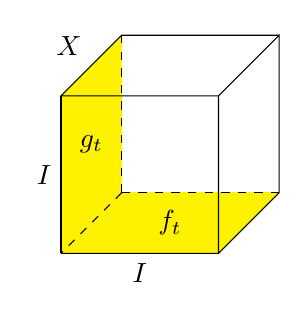
\begin{tikzpicture}[scale=2]
\filldraw [yellow] (0,0,0)--(0,0,1)--(0,1,1)--(0,1,0)--cycle;
\filldraw [yellow] (0,0,0)--(0,0,1)--(1,0,1)--(1,0,0)--cycle;
\draw[dashed] (0,0,0)--(1,0,0);
\draw[dashed] (0,0,0)--(0,1,0);
\draw[dashed] (0,0,0)--(0,0,1);
\draw (0,0,1)--(1,0,1)--(1,1,1)--(1,1,0)--(1,0,0)--(1,0,1);
\draw (1,1,1)--(0,1,1)--(0,1,0)--(1,1,0);
\draw (0,1,1)--(0,0,1);
\node at (0,0.5,0.5) {$g_t$};
\node at (0.5,0,0.5) {$f_t$};
\node at (0,1,0.5)[above left] {$X$};
\node at (0,0.5,1)[left] {$I$};
\node at (0.5,0,1)[below] {$I$};
\end{tikzpicture}
\end{center}
Need $h(x,s)=H(x,0,s)$, $f(x,t)=H(x,t,0)$, $g(x,t)=H(x,t,1)$ so that $h(x,0)=f(x,0)$, $h(x,1)=g(x,0)$
\begin{center}
\begin{tikzcd}
X \arrow[r, "h"] \arrow[d, hook]                            & Y^I \arrow[d] \\
X\times I \arrow[r, "{(f_t,g_t)}"'] \arrow[ru, "H", dashed] & Y\times Y    
\end{tikzcd}
\end{center}
$X\times I^2$ can be deformed onto $X\times I\cup X\times I\cup X\times I=X\times (I\cup I\cup I)$
\begin{center}
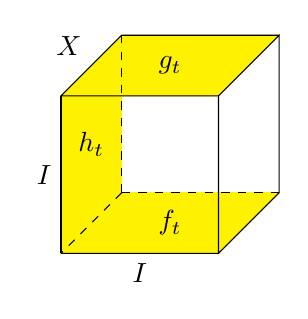
\begin{tikzpicture}[scale=2]
\filldraw [yellow] (0,0,0)--(0,0,1)--(0,1,1)--(0,1,0)--cycle;
\filldraw [yellow] (0,0,0)--(0,0,1)--(1,0,1)--(1,0,0)--cycle;
\filldraw [yellow] (0,1,0)--(0,1,1)--(1,1,1)--(1,1,0)--cycle;
\draw[dashed] (0,0,0)--(1,0,0);
\draw[dashed] (0,0,0)--(0,1,0);
\draw[dashed] (0,0,0)--(0,0,1);
\draw (0,0,1)--(1,0,1)--(1,1,1)--(1,1,0)--(1,0,0)--(1,0,1);
\draw (1,1,1)--(0,1,1)--(0,1,0)--(1,1,0);
\draw (0,1,1)--(0,0,1);
\node at (0,0.5,0.5) {$h_t$};
\node at (0.5,0,0.5) {$f_t$};
\node at (0.5,1,0.5) {$g_t$};
\node at (0,1,0.5)[above left] {$X$};
\node at (0,0.5,1)[left] {$I$};
\node at (0.5,0,1)[below] {$I$};
\end{tikzpicture}
\end{center}
\end{solution}

\begin{exercise}\label{U<R^n open, boundary point is the limit of some discrete sequence}
$U\subsetneqq\mathbb R^n$ is a nonempty open set, $x\in\partial U$, then there exists a discrete sequence $\{x_i\}\subseteq U$ converges to $x$
\end{exercise}

\begin{solution}
$x$ is necessarily an accumulation point since $\partial U\cap U=\varnothing$. Pick $x_0\in U$, then we can find $\epsilon>0$ such that $x_0\notin B(x,\epsilon)$, then pick $x_1\in B(x,\epsilon/2)\cap U$, and so on
\end{solution}

\begin{exercise}\label{f analytic near 0, after change of variables, f has terms only involve one variable}
$f$ is analytic near $0$, by rotation of coordinates, we can always make $f$ has terms only involve one variable
\end{exercise}

\begin{exercise}
Evaluate $\displaystyle\int_0^\infty e^{-s^2-\frac{1}{s^2}}ds$
\end{exercise}

\begin{solution}
$\left(s-\dfrac{1}{s}\right)^2=s^2+\dfrac{1}{s^2}-2$, let $x=s-\dfrac{1}{s}$ which is increasing on $(0,\infty)$ since $0<s<\infty$, $-\infty<x<\infty$, then $s=\dfrac{x+\sqrt{x^2+4}}{2}$ and
\[\displaystyle\int_0^\infty e^{-s^2-\frac{1}{s^2}}ds=e^{-2}\int_{-\infty}^{+\infty}e^{-x^2}\left(\dfrac{1}{2}+\dfrac{x}{2\sqrt{x^2+4}}\right)dx=e^{-2}\int_0^\infty e^{-x^2}dx=\dfrac{e^{-2}\sqrt{\pi}}{2}\]
\end{solution}

\begin{exercise}
$f$ is holomorphic on the punctured unit disc, $p>0$, $\displaystyle \int_{D}|f(z)|^pdz<\infty$. What can we say about the singularity?
\end{exercise}

\begin{solution}
$|f(z)|^p=e^{p\log|f(z)|}$ is subharmonic by Example \ref{f holomorphic => log|f| subharmonic}, thus essential singularity is impossible
\[|f(z)|^p\leq\frac{4}{\pi |z|^2}\int_{|w-z|<|z|/2}|f(w)|^pdw\leq \frac{C}{|z|^2}\]
Thus $|z|^\frac{2}{p}|f(z)|<\infty$
\end{solution}

\begin{exercise}
$U\subseteq\Omega\subseteq\mathbb C$ are open, $f$ is holomorphic on $U$, $\widehat U_\Omega$ be the union of $U$ and compact connected components of $\Omega\setminus U$. There exist $\{f_n\}$ holomorphic on $\Omega$ converging uniformly to $f$ on compact subsets of $U$ iff there exists $g$ holomorphic on $H(\widehat U_\Omega)$ such that $g|_U=f$
\end{exercise}

\begin{solution}
Assume $\widehat U_\Omega=U\cup K_1\cup\cdots$, where $K_i$'s are compact \par
Suppose $\{f_n\}$ holomorphic on $\Omega$ converging uniformly to $f$ on compact subsets of $U$, by maximum principle, $\{f_n\}$ would be uniformly bounded around $K_i$, by Montel's theorem \ref{Montel's theorem}, there exists a subsequence of $\{f_n\}$ converges uniformly on $K_i$, thus converging to $g$ holomorphic on $H(\widehat U_\Omega)$, hence $g|_U=f$ \par
Conversely, suppose $g$ holomorphic on $H(\widehat U_\Omega)$ such that $g|_U=f$, $\widehat U_\Omega$ is simply connected, by Riemann mapping theorem \ref{Riemann mapping theorem}, we can think of $\widehat U_\Omega$ as the unit disc or $\mathbb C$, by Runge's theorem, there exist $\{f_n\}$ holomorphic on $\Omega$ uniformly converging to $g$ on each disc. Thus there exist a subsequence of $\{f_n\}$ converging uniformly to $g$ on compact subsets of $\widehat U_\Omega$
\end{solution}

\begin{exercise}
Let $\Omega$ be an open subset of $\mathbb C$, $\mathscr D=\{D_i\}$ be an open cover of $\Omega$ with disks. Given meromorphic functions $h_i$ on $D_i$, not identically zero. Assume $g_{ij}=\dfrac{h_i}{h_j}$ are holomorphic on $D_i\cap D_j$, then there exist holomorphic function $f_i$ with no zeros on $D_i$ such that $f_i=g_{ij}f_j$
\end{exercise}

\begin{solution}
It suffices to prove $H^1(\Omega,\mathcal{O}^*)=0$, since then $H^1(\mathscr D,\mathcal{O}^*)=0$, $(g_{ij})\in Z^1(\mathscr D,\mathcal O^*)=B^1(\mathscr D,\mathcal O^*)$, i.e. there exists $(f_i)\in C^0(\mathscr D,\mathcal O^*)$ such that $f_i=g_{ij}f_j$ \par
Consider exact sequence of sheaves $0\to\mathbb Z\hookrightarrow\mathcal O\xrightarrow{\exp}\mathcal O^*\to0$, then we get a long exact sequence $\cdots\to H^1(\Omega,\mathcal O)\to H^1(\Omega,\mathcal O^*)\to H^2(\Omega,\mathbb Z)\to\cdots$, $H^1(\Omega,\mathcal O)=0$ by Mittag-Leffler theorem
\end{solution}

\begin{exercise}
For each real $r$ such that $0<|r|<1$, prove that there exists at most one real $s$ with $0<s<1$ for which $\Omega:=D\setminus\{0,r,s\}$ admits an analytic automorphism different from the identity
\end{exercise}

\begin{solution}
Suppose $\Omega\xrightarrow\phi\Omega$ is an analytic automorphism, then $0,r,s$ are all removable singularities, by continuity, $\phi$ can be extended to $D\xrightarrow\phi D$, so is $\phi^{-1}$, by continuity, we know $\phi$ is an automorphism of $D$, sending $\{0,r,s\}$ to itself bijectively \par
By Schwarz lemma, we know that an automorphism $\phi$ of $D$ with $\phi(\alpha)=0$ iff $\phi=e^{i\theta}\dfrac{z-\alpha}{1-\overline\alpha z}$ \par
Now suppose $\phi$ is an automorphism different from the identity, if $0<r=s<1$, then $\phi=-\dfrac{z-r}{1-rz}$ is a choice, now we assumen $r\neq s$
\begin{enumerate}[{label=\textbf{Case \Roman*:}}, leftmargin=*, align=left]
\item $\phi(0)=0$ \par
$\phi=e^{i\theta}z$, $\phi(r)=s$, but $0<s<1$, thus $s=|r|$
\item $\phi(r)=0$ \par
$\phi=e^{i\theta}\dfrac{z-r}{1-\overline r z}$, $\phi(0)=-re^{i\theta}$
\begin{enumerate}[{label=\textbf{Case \roman*:}}, leftmargin=*, align=left]
\item $\theta=\pi$, $\phi(0)=r$, then $s=\phi(s)\Rightarrow \overline rs^2-2s+r=0\Rightarrow s=\dfrac{1+\sqrt{1-|r|^2}}{\overline r}\text{ or }\dfrac{1-\sqrt{1-|r|^2}}{\overline r}$, $r$ has to be a positive real number and $s=\dfrac{1-\sqrt{1-r^2}}{r}$
\item $s=\phi(0)=|r|$
\end{enumerate}
\item $\phi(s)=0$ \par
$\phi=e^{i\theta}\dfrac{z-s}{1-sz}$, $\phi(0)=-se^{i\theta}$
\begin{enumerate}[{label=\textbf{Case \roman*:}}, leftmargin=*, align=left]
\item $\theta=\pi$, $\phi(0)=s$, then $r=\phi(r)\Rightarrow sr^2-2r+s=0\Rightarrow s=\dfrac{2r}{1+r^2}$.
\item $r=\phi(0)=-se^{i\theta}$, $s=\phi(r)\Rightarrow s^2=1$ which is impossible
\end{enumerate}
\end{enumerate}
\end{solution}

\begin{exercise}
$F\subseteq\mathbb C$ is closed, connected and noncompact, $\Omega=\mathbb C\setminus F$, then every $f\in\mathcal O(\Omega)$ has a primitive
\end{exercise}

\begin{solution}
It suffices to show that every connected component $U$ of $\Omega$ is simply connected \par
Suppose $U$ is not simply connected, then $\pi_1(U,z_0)\neq0$, i.e. there is a simple(self non-intersecting) loop $\gamma\subseteq U$ with $\gamma(0)=\gamma(1)$ cannot be deform to $z_0$, by Jordan curve theorem \ref{Jordan curve theorem}, $\gamma$ divides $\mathbb C$ into the exterior and the interior which is homeomorphic to the unit disc $D$, suppose $F\cap D$ is empty, then $\overline D\subseteq U$, $\gamma$ can be deformed to $z_0$, giving a contradiction, hence $F\cap\overline D$ is a compact connected component of $F$ which is also a contradiction
\end{solution}

\begin{exercise}
Consider an open set $\Omega\subseteq\mathbb C^2$ such that
\[\{(z,w)\in\mathbb C^2||z|\leq R_1,|w|\leq R_2\}\subseteq\Omega\]
for some positive reals $R_1$ and $R_2$. Let $f\in\mathcal H(\Omega)$ be such that $f(z,w)\neq0$ for every $z$ and $w$ for which $|z|\leq R_1$, $|w|=R_2$
\begin{enumerate}[label=\textbf{\arabic*.}, leftmargin=*]
\item Prove that the number (counted with multiplicities) of zeros of $w\mapsto f(z,w)$ in $D(0,R_2)$ is the same for every $|z|\leq R_1$
\item Let $w_1(z),\cdots,w_m(z)$ denote the zeros of $w\mapsto f(z,w)$ (counted with multiplicities). Prove that for each $n\in\mathbb N$ the function
\[z\mapsto w_1(z)^n+\cdots+w_m(z)^n\]
is holomorphic for $z\in D(0,R_1)$
\item Deduce that $n$th elementary symmetric function $\sigma_n$ of $w_1(z),\cdots,w_m(z)$ is holomorphic. \par
\item Prove that there exists a function $h$ that is holomorphic and without any zeros on $\{(z,w)\in\mathbb C^2||z|< R_1,|w|< R_2\}$ such that
\[f(z,w)=h(z,w)[w^m+\sigma_1(z)w^{m-1}+\cdots+\sigma_{m-1}(z)w+\sigma_m(z)]\]
for every $z$ and $w$ such that $|z|<R_1$ and $|w|<R_2$
\end{enumerate}
\end{exercise}

\begin{solution}
\begin{enumerate}[label=\textbf{\arabic*.}, leftmargin=*]
\item By Lemma \ref{Lemma for finding zeros}, $\displaystyle\frac{1}{2\pi i}\int_{\partial D(0,R_2)}\frac{f_w(z,w)}{f(z,w)}dw$ is the number of zeros in $D(0,R_2)$ which is continuous, hence the same for every $|z|\leq R_1$
\item By Lemma \ref{Lemma for finding zeros}, $\displaystyle\frac{1}{2\pi i}\int_{\partial D(0,R_2)}w^n\frac{f_w(z,w)}{f(z,w)}dw=w_1(z)^n+\cdots+w_m(z)^n$ is holomorphic
\item Directly follows from (2) thanks to Newton's identities
\item Since $\displaystyle\prod_{i=1}^m(w-w_i(z))=w^m+\sigma_1(z)w^{m-1}+\cdots+\sigma_{m-1}(z)w+\sigma_m(z)$ is holomorphic
\[\dfrac{f(z,w)}{w^m+\sigma_1(z)w^{m-1}+\cdots+\sigma_{m-1}(z)w+\sigma_m(z)}\]
has no zeros on $D$ and holomorphic on $\{R_2-\varepsilon<|w|<R_2\}$, hence by Hartogs's extension theorem \ref{Hartogs's extension theorem}, can be extended to a holomorphic function $h(z,w)$, then $f(z,w)=h(z,w)[w^m+\sigma_1(z)w^{m-1}+\cdots+\sigma_{m-1}(z)w+\sigma_m(z)]$ on $\{R_2-\varepsilon<|w|<R_2\}$, by identity theorem, this holds for all $|z|<R_1$ and $|w|<R_2$
\end{enumerate}
\end{solution}

\begin{exercise}
Suppose $p_1,\cdots,p_n$ are points on the compact Riemann surface $X$ and $X'=X\setminus\{p_1,\cdots, p_n\}$. Suppose $f:X'\to\mathbb C$ is a non-constant holomorphic function. Show that the image of $f$ comes arbitrarily close to every $c\in\mathbb C$
\end{exercise}

\begin{solution}
Suppose there exists $c\in\mathbb C$ such that $|f-c|\geq\varepsilon$ for some $\varepsilon>0$, then $\dfrac{1}{f-c}$ would be a bounded holomorphic function on $X'$, by Riemann's Removable singularity theorem, $\dfrac{1}{f-c}$ can be extended to a holomorphic function on $X$, but since $X$ is compact, $\dfrac{1}{f-c}$ is a constant which is impossible
\end{solution}

\begin{exercise}
Let $X$ be a compact Riemann surface and let $X\xrightarrow\sigma X$ be a biholomorphic map of $X$ onto itself, different from the identity. Let $a\in X$ be a point with $\sigma(a)\neq a$, and suppose that there is a non-constant meromorphic function $f$ on $X$, holomorphic on $X\setminus\{a\}$, with a pole of order $k$ at $a$. Prove that $\sigma$ can have at most $2k$ fixed points on $X$
\end{exercise}

\begin{solution}
Suppose there are more than $2k$ fixed points of $\sigma$, then consider $f-f\circ\sigma^{-1}: X\rightarrow\mathbb{P}^1$ is holomorphic on $X\setminus\{a,\sigma^{-1}(a)\}$ with at least $2k+1$ zeros and with poles of order $k$ at $a, \sigma^{-1}(a)$, but it should have as many poles as zeros which is a contradiction
\end{solution}

\begin{exercise}
$\Lambda=\mathbb Z\omega_1+\mathbb Z\omega_2$ and $\Lambda'=\mathbb Z\omega_1'+\mathbb Z\omega_2'$ are lattices in $\mathbb C$. Show that $\Lambda=\Lambda'$ iff there exists a matrix $A\in GL(2,\mathbb Z)$ such that
\[\begin{pmatrix}
\omega_1' \\
\omega_2'
\end{pmatrix}=A\begin{pmatrix}
\omega_1 \\
\omega_2
\end{pmatrix}\]
\end{exercise}

\begin{solution}
First not that
\[
\Lambda \subseteq \Lambda' \quad \Leftrightarrow \quad 
\begin{pmatrix}
\omega_{1}\\ 
\omega_{2}
\end{pmatrix}
=A
\begin{pmatrix}
\omega_{1}'\\ 
\omega_{2}'
\end{pmatrix}
\text{    for some    } A \in \mathrm{M}(2,\mathbb{Z})
\]
Hence we have
\[
\Lambda = \Lambda' \quad \Leftrightarrow \quad 
\begin{pmatrix}
\omega_{1}\\ 
\omega_{2}
\end{pmatrix}
=A
\begin{pmatrix}
\omega_{1}'\\ 
\omega_{2}'
\end{pmatrix}
,
\begin{pmatrix}
\omega_{1}'\\ 
\omega_{2}'
\end{pmatrix}
=B
\begin{pmatrix}
\omega_{1}\\ 
\omega_{2}
\end{pmatrix}
\text{    for some    }A,B \in \mathrm{M}(2,\mathbb{Z})
\]
Which is equivalent to \(A\in \mathrm{GL}(2,\mathbb{Z})\)
\end{solution}

\begin{exercise}
$\Lambda=\mathbb Z\omega_1+\mathbb Z\omega_2$, $\Lambda'=\mathbb Z\omega_1'+\mathbb Z\omega_2'$ are lattices in $\mathbb C$ and $X=\mathbb C/\Lambda$, $X'=\mathbb C/\Lambda'$ are the corresponding complex tori
\begin{enumerate}[label=\textbf{\arabic*.}, leftmargin=*]
\item Prove that any holomorphic map $X\xrightarrow f X'$ is induced by a linear map $\mathbb C\xrightarrow g\mathbb C$ of the form $g(z)=\alpha z + \beta$, where
$\alpha\in \mathbb C$ is such that $\alpha\Lambda\subseteq \Lambda'$. $f$ is biholomorphic if and only if $\alpha\Lambda = \Lambda'$
\item Show that every torus $X=\mathbb C/\Lambda$ is isomorphic to a torus of the form $X(\tau)=\mathbb C/(\mathbb Z+\mathbb Z\tau)$, where $\tau\in\mathbb C$ satisfies $\mathrm{Im}(\tau)>0$
\item Assume that $\left(\begin{array}{cc} a & b \\ c &
  d \end{array}\right)\in\mathrm{SL}(2,\mathbb Z)$ and $\mathrm{Im}(\tau)>0$. Let $\displaystyle \tau':=\frac{a\tau + b}{c\tau +d}$. Show that the tori $X(\tau)$ and $X(\tau')$ are biholomorphic
\end{enumerate}
\end{exercise}

\begin{solution}
\begin{enumerate}[label=\textbf{\arabic*.}, leftmargin=*]
\item Since $\mathbb{C}$ is the universal cover of \(\mathbb{C}/\Lambda'\), $f\circ\pi:\mathbb{C}\rightarrow \mathbb{C}/\Lambda'$ has a lift $F:\mathbb{C}\rightarrow \mathbb{C}$, and locally we have $F=\pi'|_{V}^{-1}\circ f\circ\pi|_{U}$, thus $F$ is holomorphic
\begin{center}
\begin{tikzcd}
&\mathbb{C} \arrow[r,"F"] \arrow[d,"\pi"]
& \mathbb{C} \arrow[d,"\pi'"] \\
& \mathbb{C}/\Lambda \arrow[r,"f"]
& \mathbb{C}/\Lambda'
\end{tikzcd}
\end{center}
Fix \(\omega\in \Lambda\), since $\pi(z+\omega)=\pi(z)$ for any $z\in \mathbb{C}$, we have $F(z+\omega)-F(z)\in\Lambda'$, hence  \(F(z+\omega)-F(z)\) is a continuous function of $z$ but $\Lambda'$ is discrete, thus $F(z+\omega)-F(z)\equiv C_{\omega}$, where $C_{\omega}\in\Lambda'$ is a constant. Then $F'(z+\omega)=F'(z)$ which shows $F':\mathbb{C}\rightarrow \mathbb{C}$ is doubly periodic function, thus induces $G:\mathbb{C}/\Lambda\rightarrow \mathbb{C}$ with $F=G\circ\pi$. Thus $G$ must be a constant, so is $F'$, therefore $F$ has the form $F(z)=\alpha z+\beta$. Then for any $\omega\in \Lambda$, we have $F(\omega)-F(0)=\alpha\omega\in\Lambda'$, thus $\alpha\Lambda\subset\Lambda'$. If $f$ is biholomorphic, then $\pi'\circ F=f\circ\pi\Rightarrow \pi\circ F^{-1}=f^{-1}\circ\pi'$, which implies $\left\{\begin{array}{rl}
\alpha\Lambda\subset\Lambda' \\
\alpha^{-1}\Lambda'\subset\Lambda
\end{array}\right. \Rightarrow \alpha\Lambda=\Lambda'$
\begin{center}
\begin{tikzcd}
&\mathbb{C} \arrow[d,"\pi"]
& \mathbb{C} \arrow[l,"F^{-1}"] \arrow[d,"\pi'"] \\
& \mathbb{C}/\Lambda
& \mathbb{C}/\Lambda' \arrow[l,"f^{-1}"]
\end{tikzcd}
\end{center}
Conversely, if \(\alpha\Lambda=\Lambda'\), $\pi\circ F^{-1}$ is doubly periodic and induce $f^{-1}$, hence $f$ is biholomorphic
\item Suppose $\Lambda=\mathbb{Z}\omega_{1}+\mathbb{Z}\omega_{2}, \mathrm{Im}\left(\dfrac{\omega_{2}}{\omega_{1}}\right)>0$, define $\Lambda'=\mathbb{Z}+\mathbb{Z}\tau$, where $\tau=\dfrac{\omega_{2}}{\omega_{1}}$, we have $\omega_{1}\Lambda'=\Lambda$, thus $X$ and $X(\tau)$ are biholomorphic
\item $X(\tau)$ and $X(\tau')$ are biholomorphic iff $\begin{pmatrix}
\tau'\\ 
1
\end{pmatrix}
=\alpha A
\begin{pmatrix}
\tau\\ 
1
\end{pmatrix}, \alpha\in \mathbb{C}-\{0\}, A\in \mathrm{SL}(2,\mathbb{Z})$
If $X(\tau)$ and $X(\tau')$ are biholomorphic, then $\mathbb{Z}+\mathbb{Z}\tau'=\Lambda'=\alpha\Lambda=\mathbb{Z}\alpha+\mathbb{Z}\alpha\tau$ for some $\alpha\in \mathbb{C}-\{0\}$, thus $\begin{pmatrix}
\tau'\\ 
1
\end{pmatrix}
=
A
\begin{pmatrix}
\alpha\tau\\ 
\alpha
\end{pmatrix}
=\alpha A
\begin{pmatrix}
\tau\\ 
1
\end{pmatrix}$, for some $A\in \mathrm{SL}(2,\mathbb{Z})$, the other direction is easy
\end{enumerate}
\end{solution}

\begin{exercise}
Determine the branch points(or ramification points) of the map $f:\mathbb C\to\mathbb P^1$ with
\[f(z)=\frac{1}{2}\left(z+\frac{1}{z}\right)\]
\end{exercise}

\begin{solution}
$f'(z)=\dfrac{1}{2}\left(1-\dfrac{1}{z^{2}}\right)$ when $z\neq0$, thus $1,-1$ are branch points. \par
Consider the chart $({P}^{1}-\{0\},\varphi)$ with $\varphi(z)=\dfrac{1}{z}$

\begin{center}
\begin{tikzcd}
\mathbb{C} \arrow[r,"f"] \arrow[dr]
& \mathbb{P}^{1}-\{0\} \arrow[d,"\varphi"] \\
& \mathbb{C}
\end{tikzcd}
\end{center}

Thus $g(z)=\varphi\circ f(z)=\dfrac{z}{2(z^{2}+1)}$, $g'(z)=\dfrac{1-z^{2}}{2(z^{2}+1)}$, hence \(0\) is not a branch point
\end{solution}

\begin{exercise}
If $f$ and $g$ are two elliptic functions with respect to the same lattice $\Omega\subseteq\mathbb C$, prove that there exists an irreducible polynomial $P(x,y)\in \mathbb C[x,y]$ such that $P(f,g)=0$
\end{exercise}

\begin{solution}
If $f\equiv c$ is a constant, then $P(x,y)=x-c$ is an irreducible polynomial such that $P(f,g)=0$, so we can assume $f,g$ are not constants, Since $\mathcal{M}(X)$ is a finite algebraic extension of $\mathbb{C}(f)$, there exists rational functions $R_0,\cdots,R_n$ such that $R_0(f)+R_1(f)g+\cdots+R_n(f)g^n=0$, then after multiplying denominators, we get a polynomial $P(x,y)\in \mathbb{C}[x,y]$ such that $P(f,g)=0$, since $\mathbb{C}[x,y]$ is a UFD, $P=P_1\cdots P_k$, where $P_i$ are prime hence irreducible, then $0=P_1(f,g)\cdots P_k(f,g)\in \mathcal{M}(X)$ which is a field, thus $P_j(f,g)=0$ for some irreducible polynomial $P_j\in \mathbb{C}[x,y]$ 
\end{solution}

\begin{exercise}
$f$ is an elliptic function of order $n>0$, then $f'$ is an elliptic function of order $m$ such that $n+1\leq m \leq 2n$. Both bounds can be attained
\end{exercise}

\begin{solution}
$f'$ is elliptic since $f(z+\omega)=f(z)\Rightarrow f'(z+\omega)=f'(z)$ for all $\omega\in\Omega$. Suppose $f$ has poles $[P_1],\cdots,[P_{k}]$ with multiplicities $r_1,\cdots,r_k$, $\sum r_i=n$, then $f'$ also has poles $[P_1],\cdots,[P_{k}]$ with multiplicities $r_1+1,\cdots,r_k+1$, $\sum r_i=n+k=m$, since $1\leq k\leq n$, $n+1\leq m\leq 2n$ \par
We can find an elliptic function $f$ of order $n$ which has $[P_1],\cdots,[P_{n-m}]$ as its poles with multiplicities $1,\cdots,1,2n+1-m$, then we get $f'$ is another elliptic function which also has $[P_1],\cdots,[P_{n-m}]$ as its poles with multiplicities $2,\cdots,2,2n+2-m$, thus $f'$ is of order $m$
\end{solution}

\begin{exercise}
Prove that 
\[
\wp'(z) = \frac{2\,\sigma(z-\frac{\omega_1}{2})\,
\sigma(z-\frac{\omega_2}{2})\,\sigma(z-\frac{\omega_3}{2})}
{\sigma(\frac{\omega_1}{2})\,\sigma(\frac{\omega_2}{2})\,
\sigma(\frac{\omega_3}{2})\,\sigma(z)^3}\,.
\]
\end{exercise}

\begin{solution}
$\wp'(z)$ has a pole at $z=0$ of order $3$ and $\dfrac{\omega_1}{2},\dfrac{\omega_2}{2},\dfrac{\omega_3}{2}$ as simple roots, thus \[
\wp'(z)=\lambda\dfrac{\sigma\left(z-\frac{\omega_1}{2}\right)\sigma\left(z-\frac{\omega_2}{2}\right)\sigma\left(z-\frac{\omega_3}{2}\right)}{\sigma(z)^3}\]
for some $\lambda\in\mathbb{C}$, multiply by $z^3$ on both sides, and let $z\rightarrow 0$, since $\displaystyle\lim_{z\rightarrow 0}\dfrac{z}{\sigma(z)}=1, \lim_{z\rightarrow 0}z^3\wp'(z)=-2$, we have
\[-2=-\lambda\sigma\left(\dfrac{\omega_1}{2}\right)\sigma\left(\dfrac{\omega_2}{2}\right)\sigma\left(\dfrac{\omega_3}{2}\right)\Rightarrow \lambda=\dfrac{2}{\sigma\left(\frac{\omega_1}{2}\right)\sigma\left(\frac{\omega_2}{2}\right)\sigma\left(\frac{\omega_3}{2}\right)}\]
Hence
\[\wp'(z)=\dfrac{2\sigma\left(z-\frac{\omega_1}{2}\right)\sigma\left(z-\frac{\omega_2}{2}\right)\sigma\left(z-\frac{\omega_3}{2}\right)}{\sigma\left(\frac{\omega_1}{2}\right)\sigma\left(\frac{\omega_2}{2}\right)\sigma\left(\frac{\omega_3}{2}\right)\sigma(z)^3}\]
\end{solution}

Let $\Omega\subseteq \mathbb C$ be a lattice and $\wp(z)$ the associated Weierstrass $\wp$-function. We have seen that $\wp(z)$ satisfies the differential equation $(\wp'(z))^2 = p(\wp(z))$, where $p(x) = 4x^3-g_2x-g_3$. The following three problems examine the conditions under which the coefficients $g_2$ and $g_3$ of $p(x)$ are real numbers

\begin{exercise}
Prove that the following conditions are equivalent
\begin{enumerate}[label=(\roman*), leftmargin=*, align=left]
\item $g_2,g_3\in\mathbb R$
\item $G_k\in \mathbb R$ for all $k\geq 3$
\item $\wp(\bar z) = \overline{\wp(z)}$ for all $z\in\mathbb C$
\item $\overline{\Omega} = 
\Omega$ (the last condition says that $\Omega$ is a \textit{real lattice})
\end{enumerate}
\end{exercise}

\begin{solution}
$(i)\Rightarrow(ii)$ \par
$g_2=60G_4,g_3=140G_6\in\mathbb{R}\Rightarrow G_4,G_6\in\mathbb{R}$ \par
Since
\begin{align*}
\wp(z)&=\dfrac{1}{z^2}+\sum_{n=2}^{\infty}(2n-1)G_{2n}z^{2n-2} \\
&=\dfrac{1}{z^2}+3G_4z^2+5G_6z^4+7G_8z^6+9G_{10}z^8+\cdots
\end{align*}
\begin{align*}
\wp'(z)&=-\dfrac{2}{z^3}+\sum_{n=2}^{\infty}(2n-1)(2n-2)G_{2n}z^{2n-3} \\
&=-\dfrac{2}{z^3}+6G_4z+20G_6z^3+42G_8z^5+72G_{10}z^7+\cdots
\end{align*}
\begin{align*}
\wp''(z)&=\dfrac{6}{z^4}+\sum_{n=2}^{\infty}(2n-1)(2n-2)(2n-3)G_{2n}z^{2n-4} \\
&=\dfrac{6}{z^4}+6G_4+60G_6z^2+210G_8z^4+504G_{10}z^6+\cdots
\end{align*}
So we can conclude $\wp''(z)-6\wp(z)^2+30G_4=z\varphi(z)$, where $\varphi(z)$ is a holomorphic elliptic function, hence $\wp''(z)-6\wp(z)^2+30G_4=0$, then the coefficients of $z^{2n}(n\geq 1)$ would be $(2n+1)(2n+2)(2n+3)(2n+4)G_{2n+4}-6(2n+3)G_{2n+4}$ minus terms only involving $G_4,G_6,\cdots,G_{2n+2}$ and real numbers, thus by induction, we know $G_{2n+4}\in\mathbb{R}(n\geq 1)$ \par
$(ii)\Rightarrow(iii)$ \par
Since $\wp(z)=\dfrac{1}{z^2}+\sum_{n=2}^{\infty}(2n-1)G_{2n}z^{2n-2}$, if $G_k\in\mathbb{R}(k\geq 3)$, then $\wp(\bar{z})=\overline{\wp(z)}$ \par
$(iii)\Rightarrow(iv)$ \par
The poles of $\overline{\wp(\bar{z})}=\wp(z)$ are exactly $\overline{\Omega}$, thus $\overline{\Omega}=\Omega$ \par
$(iv)\Rightarrow(i)$ \par
$\displaystyle g_2=60G_4=60\sum_{\omega\in\Omega^*}\dfrac{1}{\omega^4}=60\sum_{\omega\in\overline{\Omega}^*}\dfrac{1}{\omega^4}=\overline{g_2}\Rightarrow g_2\in\mathbb{R}$, similarly, $g_6\in\mathbb{R}$
\end{solution}

\begin{exercise}
We say that $\Omega$ is {\em real rectangular} if $\Omega = \mathbb Z\omega_1+\mathbb Z\omega_2$ where $\omega_1\in \mathbb R$ and $\omega_2\in i\mathbb R$, and that $\Omega$ is {\em real rhombic} if $\Omega = \mathbb Z\omega_1+\mathbb Z\omega_2$ where $\omega_2 = \overline{\omega}_1$. Prove that a lattice $\Omega$ is real if and only if it is real rectangular or real rhombic
\end{exercise}

\begin{solution}
If $\Omega$ is real rectangular or real rhombic, $\Omega$ is obviously a real lattice \par
Conversely, if $\Omega$ is a real lattice, suppose $\Omega=\mathbb{Z}\omega_1+\mathbb{Z}\omega_2$, then there exists $\omega\in\Omega\setminus(\mathbb{R}\cup i\mathbb{R})$, otherwise, $\omega_1\in\mathbb{R}^*,\omega_2\in i\mathbb{R}^*$ or $\omega_2\in\mathbb{R}^*,\omega_1\in i\mathbb{R}^*$, since $\omega_1,\omega_2$ are linear independent, but then $\omega=\omega_1+\omega_2\in\Omega\setminus(\mathbb{R}\cup i\mathbb{R})$ which is a contradiction \par
Since $\omega\in\Omega\setminus(\mathbb{R}\cup i\mathbb{R})$, $\omega+\overline{\omega}\in\mathbb{R}^*,\omega-\overline{\omega}\in i\mathbb{R}^*$, thus $\Omega\cap\mathbb{R}^*\neq\varnothing,\Omega\cap i\mathbb{R}^*\neq\varnothing$, let $\displaystyle\eta_1=\min_{\eta\in\Omega\cap(0,\infty)}\eta$, then $\Omega\cap\mathbb{R}=\mathbb{Z}\eta_1$, otherwise $\exists \eta\in \mathbb{R}\setminus\mathbb{Z}\eta_1$, then $\eta-\left\lfloor\frac{\eta}{\eta_1}\right\rfloor\eta_1\in\Omega\cap(0,\infty)$ which is a contradiction \par
Similarly, $\Omega\cap i\mathbb{R}=\mathbb{Z}\eta_2$ for some $\eta_2\in i(0,\infty)$. If $\Omega=\mathbb{Z}\eta_1+\mathbb{Z}\eta_2$, then $\Omega$ is real rectangular, if not, $\exists \gamma\in\Omega\setminus(\mathbb{R}\cup i\mathbb{R})$, such that $\displaystyle|\gamma|=\min_{\omega\in\Omega\setminus(\mathbb{R}\cup i\mathbb{R})}|\omega|$, then $\gamma+\overline{\gamma}=\eta_1$ or $-\eta_1$, otherwise $\gamma+\overline{\gamma}=k\eta_1$ for some $|k|\geq 2$ \par
If $k=2$, then $\gamma-\eta_1=\eta_1-\overline{\gamma}=-\overline{(\gamma-\eta_1)}\Rightarrow \gamma-\eta_1\in i\mathbb{R}\Rightarrow \gamma\in\mathbb{Z}\eta_1+\mathbb{Z}(\gamma-\eta_1)\subseteq\mathbb{Z}\eta_1+\mathbb{Z}\eta_2$ \par
If $k>2$, then $\gamma-\eta_1\notin \mathbb{R}\cup i\mathbb{R}$ and $|\gamma-\eta_1|<|\gamma|$, similarly for $k\leq -2$, these are all contradictions \par
Similarly, we know that $\gamma-\overline{\gamma}=\eta_2$ or $-\eta_2$ \par
Now, for any $\omega\in\Omega\setminus(\mathbb{R}\cup i\mathbb{R})$, $\omega+\overline{\omega}=k\eta_1=k(\gamma+\overline{\gamma})$ for some $k\neq 0$, then $\omega-k\gamma=k\overline{\gamma}-\overline{\omega}=-\overline{(\omega-k\gamma)}\Rightarrow \omega-k\gamma\in i\mathbb{R}$, if $\omega\neq k\gamma$, then $\omega-k\gamma=l\eta_2=l(\gamma-\overline{\gamma})\Rightarrow \omega\in \mathbb{Z}\gamma+\mathbb{Z}\overline{\gamma}$, therefore, we have $\Omega=\mathbb{Z}\gamma+\mathbb{Z}\overline{\gamma}$, $\Omega$ is real rhombic
\end{solution}

\begin{exercise}
Let $\Omega$ be a real lattice. Define the real elliptic curve $E_{\mathbb R}$ to be the set $\{(x,y)\in\mathbb R^2 \ |\ y^2=
p(x)\}$. Prove that $E_{\mathbb R}$ has one or two connected components as $\Omega$ is real rhombic or real rectangular, respectively
\end{exercise}

\begin{solution}
The number of connected components of $E_\mathbb{R}$ is one or two if $p(x)=0$ has one real root and two nonreal conjugate complex roots or three distinct real roots correspondingly \par
Since $\dfrac{\omega_1}{2},\dfrac{\omega_2}{2},\dfrac{\omega_3}{2}$ are simple roots of $\wp'(z)$, the three simple roots of $p(x)$ are $\wp\left(\dfrac{\omega_1}{2}\right),\wp\left(\dfrac{\omega_2}{2}\right),\wp\left(\dfrac{\omega_3}{2}\right)$, since $\Omega$ is a real lattice, $G_k\in\mathbb{R}$ and $\wp(z)=\dfrac{1}{z^2}+\sum_{n=2}^{\infty}(2n-1)G_{2n}z^{2n-2}$ \par
If $\Omega$ is real rectangular, then $\wp\left(\dfrac{\omega_1}{2}\right),\wp\left(\dfrac{\omega_2}{2}\right)$ are both real, thus $E_\mathbb{R}$ has two connected components \par
If $\Omega$ is real rhombic, then $\wp\left(\dfrac{\omega_3}{2}\right)$ is real $\wp\left(\dfrac{\omega_1}{2}\right)\neq\wp\left(\dfrac{\omega_2}{2}\right)$ are nonreal conjugate, thus $E_\mathbb{R}$ has only one connected component
\end{solution}

\begin{exercise}\label{Complex structures on an open annulus}
$A(r,R)=\{r<|z|<R\}$ is biholomorphic to $\{s<|z|<S\}$ iff $R/r=S/s$, $r$ can be $0$, $R$ can be $\infty$, but not at the same time
\end{exercise}

\begin{solution}
By scaling or inversion we can assume $r=s=1$ and $|f(z)|\to1$ as $|z|\to1$. Suppose $f:A(r,R)\to A(s,S)$ is a biholomorphism, then consider the Laurent series $f=\displaystyle\sum_{k=-\infty}^{\infty}c_kz^k$, for $1<t<R$, by Stokes theorem we have
\begin{align*}
A(t)&=\dfrac{1}{2i}\int_{f(\{|z|=t\})}\bar zdz=\dfrac{1}{2i}\int_{|z|=t}\overline{f(z)}df(z)=\dfrac{1}{2i}\int_{|z|=t}\overline{f(z)}f'(z)dz=\pi\sum_{k\in\mathbb Z}k|c_k|^2t^{2k}
\end{align*}
As $t\to1$, we have $A(t)\to\pi\Rightarrow\sum k|c_k|^2=1$, thus
\[A(t)-\pi t^2=\pi t^2\sum_{k\in\mathbb Z}k|c_k|^2\left(t^{2k-2}-1\right)\geq0\]
Thus $A(t)\geq\pi t^2$, as $t\to R$, $A(t)\to\pi S^2\geq\pi R^2\Rightarrow S\geq R$. Therefore we have $S=R$
\end{solution}

\begin{exercise}
Let $\mu:\mathcal B(\mathbb R)\to\mathbb R^+$ be a $\sigma$-additive set function defined on the Borel $\sigma$-algebra on $\mathbb R$ and let $D\subseteq\mathbb R$ be a discrete set with the property $x\in D$ if and only if there exists an open set $U$ such that $x\in U$ and $\mu(U)>0$. Show that $\mu$ can be expressed as a countable linear combination of measures of the form
\[\delta_x(A)=\begin{cases}
1&x\in A \\
0&x\notin A
\end{cases}\]
Where $x\in D$ and $A\in\mathcal B(\mathbb R)$
\end{exercise}

\begin{proof}
For each $x\in D$, denote $\mu(\{x\})=c_x$. Since $D$ is discrete, it is countable and any subset of $D$ is closed. For any open set $V$ in $\mathbb R$, by definition, $\mu(V-D)=0$ since $V-D$ is an open set which doesn't intersect $D$. Hence
\[\mu(V)=\mu(V\cap D)+\mu(V-D)=\mu(V\cap D)=\sum_{x\in V\cap D}c_x=\sum_{x\in D}c_x\delta_x(V)\]
i.e. $\mu$ can be expressed as a countable linear combination of Dirac measures
\end{proof}

\begin{exercise}
Let $c:[0,1]\to[0,1]$ denote the Cantor (ternary) function (known also as the Devil’s staircase, or the Cantor-Lebesgue function). For each continuous real-valued function $f : [0, 1] \to \mathbb R$, let $l(f)$ denote the Riemann integral
\[l(f) = \int_0^1f(c(x))dx\]
Find explicitly a Borel measure $\mu : \mathcal B([0, 1]) \to\mathbb R$ so that
\[l(f)=\int_{[0,1]}fd\mu\]
where $\mathcal B([0, 1])$ denotes the Borel $\sigma$-algebra over $[0, 1]$
\end{exercise}

\begin{proof}
Write $m$ as the Lebesgue measure. Since $c$ is a continuous function, the pushforward measure $\mu(E)=m(c^{-1}(E))$ is a Borel measure on $\mathcal B([0,1])$. Note that
\[\int_{[0,1]}\chi_Ed\mu=\mu(E)=m(c^{-1}(E))=\int_0^1\chi_E(c(x))dx\]
and continuous functions are approximated by simple functions, thus
\[\int_{[0,1]}fd\mu=\int_0^1f(c(x))dx\]
\end{proof}

\begin{exercise}
Suppose $f(z)$ is a meromorphic function on $\mathbb C$ with finitely many zeros and poles at $\{z_1,\cdots,z_N\}$, i.e. e. $f(z)$ is holomorphic and nowhere vanishing on $\mathbb C \setminus\{z_1,\cdots, z_N \}$.  Let $m_i\in\mathbb Z$ be the order of $f(z)$ at $z_i$. Furthermore, assume there is $A \in \mathbb C \setminus \{0\}$ and a real number $C > 0$, such that
\[|f(z)-A|\leq\frac{C}{|z|^2}\]
for all $z$ with $|z|$ sufficiently large. Prove that
\[\sum_{i=1}^Nm_iz_i=0\]
\end{exercise}

\begin{proof}
Let $w=1/z$, $g(w)=f(1/w)=f(z)$, then $|g(w)-A|\leq C|w|^2$, then $\dfrac{g(w)-A}{w^2}$ holomorphic and bounded around $0$, denote as $h(w)$, we have $g(w)=A+w^2h(w)$, hence for $R$ large enough, $\epsilon=1/R$ small enough, we have
\begin{align*}
\sum_{i=1}^Nm_iz_i&=\int_{|z|=R}z\frac{f'(z)}{f(z)}dz=\int_{|w|=\epsilon}\frac{g'(w)}{wg(w)}dw=0
\end{align*}
Since $\dfrac{g'(w)}{wg(w)}$ is holomorphic around $0$
\end{proof}

\begin{exercise}
Evaluate $\displaystyle\int_{0}^\infty\frac{\log x}{x^2+1}dx$
\end{exercise}

\begin{solution}
\begin{align*}
\int_{0}^\infty\frac{\log x}{x^2+1}dx&=\int_{-\infty}^\infty\frac{ye^y}{e^{2y}+1}dy \\
&=\int_{-\infty}^\infty\frac{y}{e^{y}+e^{-y}}dy \\
&=0
\end{align*}
\end{solution}

\begin{exercise}
Let $\{f_n\},n\geq1$ be a sequence in $L^2([0, 1])$ and $f$ be a Lebesgue measurable function such that for every Lebesgue measurable set $E$ in $[0, 1]$
\[\int_Ef_ndx\to\int_Efdx\]
as $n \to\infty$. Assume also that $\displaystyle\sup_n\int_0^1|f_n|^2dx<\infty$
\begin{enumerate}[leftmargin=*]
\item Prove that $f\in L^2([0,1])$
\item Prove that for any function $g\in L^2([0,1])$
\[\int_0^1f_ngdx\to\int_0^1fgdx\]
\end{enumerate}
\end{exercise}

\begin{solution}
\begin{enumerate}[leftmargin=*]
\item $f_n$ converge to $f$ in measure since otherwise there would exists $\epsilon>0$ and $E$ with $m(E)>0$ such that $f_n-f\geq\epsilon$ on $E$, then
\[\int_E(f_n-f)dx\geq\epsilon m(E)\]
thus there is a subsequence $f_{n_k}\to f$ almost everywhere, by Fatou's lemma
\[\int_0^1 |f|^2dx\leq\varliminf_{k\to\infty}\int_0^1|f_{n_k}|^2dx\leq\sup_{n}\int_0^1|f_{n}|^2dx<\infty\]
\item Converges in measure $\Rightarrow$ converges weakly
\begin{align*}
\int_0^1|(f_n-f)g|dx&=\int_{|f_n-f|\geq\epsilon}|f_n-f||g|dx+\int_{|f_n-f|<\epsilon}|f_n-f||g|dx \\
&\leq\|f_n-f\|_{L^2}\int_{|f_n-f|\geq\epsilon}|g|dx+\epsilon\|g\|_{L^2}
\end{align*}
\end{enumerate}
\end{solution}

\begin{exercise}
Suppose $f(z)$ is a holomorphic function on the unit disk with $|f(z)| \leq 3$ for all $|z| < 1$, and $f(1/2) = 2$. Show that $f(z)$ has no zeros in the disk $|z| < 1/8$. (Hint: first show $f(0) \neq 0$)
\end{exercise}

\begin{solution}
Consider $\phi=\dfrac{z-\frac{1}{2}}{1-\frac{1}{2}z},\psi=\dfrac{z-\frac{2}{3}}{1-\frac{2}{3}z}$, $g=\psi\circ f/3\circ\phi^{-1}\in\Aut(\mathbb D)$,then $g(0)=0$, by Schwartz lemma, $|g(z)|\leq |z|$, thus $g(-1/2)\neq-2/3\Leftrightarrow f(0)\neq0$, also it is easy to show that $\phi(\{|z|<1/8\})\subseteq\{|z|<10/17\}$, and $10/17<2,3$, $f$ has no zeros in the disk $|z|<1/8$
\end{solution}

\begin{exercise}[umd analysis qual 2021 January, problem 1]
Does there exist a Lebesgue integrable function $f : [0, +\infty) \to\mathbb R$ which is nowhere differentiable and such that the following function $F : [0, +\infty) \to\mathbb R$
\[F(x)=\int_0^xf^{2021}dm\]
where $m$ represents Lebesgue measure on $[0, +\infty)$, is well defined and infinitely differentiable? Provide an example or disprove its existence
\end{exercise}

\begin{solution}
Suppose such an $f$ exists, then $f$ is smooth since $F$ is, assume $f$ is not constantly zero, then $f=\sqrt[2021]{F}$ at where $f$ is nonzero which is smooth, giving a contradiction
\end{solution}

\begin{exercise}[umd analysis qual 2021 January, problem 2]
Let $f(z)$ be an entire function on $\mathbb C$, and suppose there is a constant $\lambda > 0$ such that for all $z \in \mathbb C$, $|\Re f(z)| \geq \lambda|\Im f(z)|$. Show that $f$ must be constant
\end{exercise}

\begin{solution}
Pick $w_0\notin\{|\Re z|\geq\lambda|\Im z|\}$, say $i$, then $\frac{1}{f-w_0}$ is bounded. $|f-i|^2\geq\frac{\lambda^2}{1+\lambda^2}>0$
\end{solution}

\begin{exercise}[umd analysis qual 2021 January, problem 3]
Let $0 < \alpha < 1$. Verify the existence of a Lebesgue measurable set $A \subseteq [0, 1]$, with the property that for every open interval $(a, b) \subset [0, 1]$, we have $m(A \cap (a, b)) = \alpha m((a, b))$? Provide an example or disprove its existence
\end{exercise}

\begin{solution}
Suppose such an $A$ exists, Let $G\supseteq A$ be a $G_\delta$ set with $m(G_\delta\setminus A)<\delta$, since $G_\delta=\bigcup I_i$ then we have
\begin{align*}
m(G_\delta)-\delta&<m(A)=\sum m(A\cap I_i)=\sum \alpha m(I_i)=\alpha m(G_\delta)\Rightarrow m(A)\leq m(G_\delta)<\frac{\delta}{1-\alpha}
\end{align*}
Since $\delta$ can be arbitrarily small, so $m(A)=0$, giving a contradiction
\end{solution}

\begin{exercise}[umd analysis qual 2021 January, problem 5]
Let $\{f_n\} \subseteq L^1_m(\mathbb R)$. Assume that the sequence $f_n$ converges to $f$ in $L^1_m(\mathbb R)$. Furthermore, assume that there exists $M > 0$ such that for all $n = 1,\cdots$, we have $\|f_n\|_2 \leq M$. Verify whether or not $f_n$ converges to $f$ in $L^p_m(\mathbb R)$ for $1 < p \leq 2$
\end{exercise}

\begin{solution}
Since $\{f_n\}$ converges to $f$ in $L^1(\mathbb R)$, there is a subsequence $f_{n_k}$ such that $f_{n_k}\to f$ almost everywhere, thus
\[\int_{\mathbb R}|f|^2dm=\int_{\mathbb R}\varliminf_k |f_{n_k}|^2dm\leq\varliminf_k\int_{\mathbb R}|f_{n_k}|^2dm\leq M^2\]
hence $f\in L^2(\mathbb R)$, by interpolation, $f,f_n\in L^p(\mathbb R)$ for $1\leq p\leq 2$, since $f_n$ is uniformally bounded, we may assume $f_{n_k}$ also weakly converges to $f$, then $f_n\to f$ in $L^1(\mathbb R)\cap L^2(\mathbb R)$, again by intepolation, $f_n\to f$ in $L^p(\mathbb R)$ for $1\leq p\leq 2$
\end{solution}

\begin{exercise}[umd analysis qual 2021 January, problem 6]
Define the following function of a complex variable $z$
\[F(z)=\int_0^\infty\frac{x^{z-1}}{e^x-1}dx\]
Show that $F(z)$ is a holomorphic function for $\Re z > 2$. Prove that $F(z)$ admits an analytic continuation as a meromorphic function for $\Re z > 0$ whose only pole is simple at $z = 1$. Compute the residue of $F(z)$ at $z = 1$
\end{exercise}

\begin{solution}
Consider $\int_\epsilon^N\frac{x^{z-1}}{e^x-1}dx$, we know that $F(z)$ is holomorphic for $\Re z>2$. Define
\[G(z)=\int_0^\infty\frac{x^{z-1}}{e^x+1}dx\]
Then
\[F(z)-G(z)=\frac{1}{2^{z-1}}F(z)\Rightarrow\left(1-\frac{1}{2^{z-1}}\right)F(z)=G(z)\]
Note that $G(z)$ is holomorphic on $\Re z>0$ and $G(1)=\ln2$. Note that
\[2^{z-1}=e^{(z-1)\ln 2}=1\iff z-1=\frac{2k\pi}{\ln2}i\]
$(1-2^{1-z})'(1+2k\pi i/\ln2)=-\ln2$, hence $\Res(F,1)=-1$
\end{solution}

\begin{remark}
Note that $F(z)=\zeta(z)\Gamma(z)$, $G(z)=\eta(z)\Gamma(z)$, here $\eta(z)$ is Dirichlet's eta function
\end{remark}

\begin{exercise}
$E\xrightarrow{p}B$ is a Serre fibration, $A\xhookrightarrow{i}X$ is a subcomplex, if either $p$ or $i$ is a weak equivalence, then we have
\begin{center}
\begin{tikzcd}
A \arrow[r, "f"] \arrow[d, "i"', hook]            & E \arrow[d, "p"] \\
X \arrow[r, "g"'] \arrow[ru, "\exists h", dashed] & B               
\end{tikzcd}
\end{center}
\end{exercise}

\begin{solution}
If $p$ is a weak equivalence, then fibers are weak contractible \par
If $i$ is a weak equivalence, then $X$ deformation retracts onto $A$
\end{solution}

\begin{exercise}\label{X1,X2 iso and Y1,Y2 iso implies Hom(X1,Y1),Hom(X2,Y2) iso}
In category $\mathscr C$, if $X\xrightarrow{\phi_X} X'$, $Y\xrightarrow{\phi_Y} Y'$ are isomorphisms, then $Hom(X,Y)$, $Hom(X',Y')$ are in bijective correspondence
\end{exercise}

\begin{solution}
Consider $Hom(X,Y)\to Hom(X',Y')$, $f\mapsto\phi_Y f\phi_X^{-1}$ and $Hom(X',Y')\to Hom(X,Y)$, $f'\mapsto\phi_Y^{-1}f'\phi_X$ which are inverses to each other
\begin{center}
\begin{tikzcd}
X \arrow[r, "f"] \arrow[d, "\phi_X"'] & Y \arrow[d, "\phi_Y"] \\
X' \arrow[r, "f'"]                  & Y'                 
\end{tikzcd}
\end{center}
\end{solution}

\begin{exercise}
Suppose the bottom row of the following commutative diagram is exact, $gf=0$, then there exists $a$ such that the following diagram commutes
\begin{center}
\begin{tikzcd}
A \arrow[r, "f"] \arrow[d, "\exists a", dashed] & B \arrow[r, "g"] \arrow[d, "b"] & C \arrow[d, "c"] \\
A' \arrow[r, "f'"]                              & B' \arrow[r, "g'"]              & C'              
\end{tikzcd}
\end{center}
\end{exercise}

\begin{solution}
Since $0=cgf=g'bf$ and bottom row is exact, we have
\begin{center}
\begin{tikzcd}
                               & A \arrow[ld, "\exists a"', dashed] \arrow[d, "bf"] \\
A' \arrow[r, "f'"', two heads] & \ker g'                                           
\end{tikzcd}
\end{center}
\end{solution}

\begin{exercise}
$F,G:\mathscr C\times\mathscr D\to\mathscr E$ are functors, $F\xrightarrow{\eta} G$ is a natural transformation iff $\eta$ is natural on each factor
\end{exercise}

\begin{solution}
We have commutative diagram
\begin{center}
\begin{tikzcd}
{F(A,B)} \arrow[r, "{F(f,1)}"] \arrow[d, "{\eta_{A,B}}"] & {F(A',B)} \arrow[r, "{F(1,g)}"] \arrow[d, "{\eta_{A',B}}"] & {F(A',B')} \arrow[d, "{\eta_{A',B'}}"] \\
{G(A,B)} \arrow[r, "{G(f,1)}"]                           & {G(A',B)} \arrow[r, "{G(1,g)}"]                            & {G(A',B')}                            
\end{tikzcd}
\end{center}
\end{solution}

\begin{exercise}\label{Fully faithfull functor is injective on objects up to isomorphism}
A fully faithful functor $F:\mathscr C\to\mathscr D$ is injective on objects up to isomorphism
\end{exercise}

\begin{solution}
Suppose $F(X)=F(Y)=T$, let $f:X\to Y$ be the map corresponds to $1_T$ in $Hom(F(X),F(Y))$, then $f:X\to Y$ is an isomorphism because we can also let $g:Y\to X$ be the map corresponds to $1_T$ as in $Hom(F(Y),F(X))$, then $F(g\circ f)=F(g)\circ F(f)=1_T\circ 1_T=1_T$, thus $g\circ f$ corresponds to $1_T$ in $Hom(F(X),F(X))$, but $F(1_X)=1_{F(X)}=1_T$, thus $g\circ f=1_X$, similarly, $f\circ g=1_Y$
\end{solution}

\begin{exercise}
Suppose $\mathscr A$ is an abelian category, show $\mathscr A$ is balanced. For any $A\xrightarrow{f}B$, $\ker f\xrightarrow{i}A$ is a monomorphism, $B\xrightarrow{\pi}\mathrm{coker}f$ is an epimorphism, and $\mathrm{im}f:=\ker\mathrm{coker}f$, $\mathrm{coim}f:=\mathrm{coker}\ker f$ are isomorphic
\end{exercise}

\begin{solution}
Suppose $A\xrightarrow{f}B$ is a bimorphism, it is the equaliser of \begin{tikzcd}
B \arrow[r, "\pi", shift left] \arrow[r, "0"', shift right] & \mathrm{coker}f
\end{tikzcd}, then $\pi=0$, $\mathrm{coker}f=0$, but $A\xrightarrow{1_A}A$ is the kernel of $A\to0$, hence $A,B$ are isomorphic \par
$\ker f\xrightarrow{i}A$ is a monomorphism due to the following diagram
\begin{center}
\begin{tikzcd}
C \arrow[d, "g=0"'] \arrow[rd, "0"'] \arrow[rrd, "0"] &                   &   \\
\ker f \arrow[r, "i"]                                 & A \arrow[r, "f"'] & B
\end{tikzcd}
\end{center}
$B\xrightarrow{\pi}\mathrm{coker}f$ is a monomorphism due to the following diagram
\begin{center}
\begin{tikzcd}
A \arrow[r, "f"] \arrow[rrd, "0"'] & B \arrow[r, "\pi"] \arrow[rd, "0"] & \mathrm{coker}f \arrow[d, "g=0"] \\
                                   &                                    & C                             
\end{tikzcd}
\end{center}
Now let's show coimage and image are isomorphic. $fi=0$ induces $\mathrm{coker}i\xrightarrow{g}B$, claim that $g$ is monic \par
Suppose $X\xrightarrow{x}\mathrm{coker}i$ is morphism such that $gx=0$, it induces $\mathrm{coker}x\xrightarrow{j}B$, since $qpk=0$, $fk=jqpk=0$ induces $\ker qp\xrightarrow{l}\ker f$, since $qp$ is epi, $pk=pil=0$ induces $\mathrm{coker}x\xrightarrow{r}\mathrm{coker}i$, since $p$ is epi, $p=rqp\Rightarrow rq=1_{\mathrm{coker}i}$, hence $q$ is monic, $qx=0\Rightarrow x=0$
\begin{center}
\begin{tikzcd}
                            & \ker qp \arrow[d, "k", tail] \arrow[ld, "l"']                         &                                                                    &                 \\
\ker f \arrow[r, "i", tail] & A \arrow[d, "p", two heads] \arrow[r, "f"]                            & B \arrow[r, "\pi", two heads]                                      & \mathrm{coker}f \\
X \arrow[r, "x"]            & \mathrm{coker}i \arrow[r, "q", two heads, shift left] \arrow[ru, "g"] & \mathrm{coker}x \arrow[l, "r", dashed, shift left] \arrow[u, "j"'] &                
\end{tikzcd}
\end{center}
$\pi f=0$ induces $A\xrightarrow{h}\ker\pi$, claim that $h$ is epi \par
Suppose $\ker\pi\xrightarrow{y}Y$ is morphism such that $yh=0$, it induces $A\xrightarrow{p}\ker y$, since $qjk=0$, $qf=qjkp=0$ induces $\mathrm{coker}f\xrightarrow{m}\mathrm{coker}jk$, since $jk$ is monic, $qj=m\pi j=0$ induces $\ker\pi\xrightarrow{s}\ker y$, since $j$ is monic, $j=jks\Rightarrow ks=1_{\ker\pi}$, hence $k$ is epi, $yk=0\Rightarrow y=0$
\begin{center}
\begin{tikzcd}
                            &                                                 & \mathrm{coker}jk                                                                &                                  \\
\ker f \arrow[r, "i", tail] & A \arrow[r, "f"] \arrow[rd, "h"] \arrow[d, "p"] & B \arrow[r, "\pi", two heads] \arrow[u, "q", two heads]                         & \mathrm{coker}f \arrow[lu, "m"'] \\
                            & \ker y \arrow[r, "k", tail, shift left]         & \ker\pi \arrow[u, "j"', tail] \arrow[r, "y"] \arrow[l, "s", dashed, shift left] & Y                               
\end{tikzcd}
\end{center}
Since $\mathrm{im}f\to B$ is monic, $A\to\mathrm{coim}f$ is epi, $g,h$ both induce $\mathrm{coim}f\xrightarrow{\phi}\mathrm{im}f$, then $\phi$ is monic and epi hence iso
\begin{center}
\begin{tikzcd}
\ker f \arrow[r, tail] & A \arrow[r, "f"] \arrow[d, two heads]    & B \arrow[r, two heads]       & \mathrm{coker}f \\
                       & \mathrm{coim}f \arrow[r, "\phi", dashed] & \mathrm{im}f \arrow[u, tail] &                
\end{tikzcd}
\end{center}
\end{solution}

\begin{exercise}\label{bounded double complex with exact rows or exact columns has exact total complex}
$C$ is a bounded double complex with exact rows or exact columns, then $Tot(C)$ is exact
\end{exercise}

\begin{solution}
Without loss of generality, we may assume $C$ is bounded in the first quadrant and has exact rows, use $d',d'',d$ to denote row, column and total differentials \par
$Tot(C)$ is exact for all $n<0$ since $Tot(C)_n=0$ for all $n<0$. now suppose $n\geq 0$, $\displaystyle d\left(\sum_{k=0}^n x_{k,n-k}\right)=0$, i.e. $d'x_{k+1,n-k-1}+d''x_{k,n-k}=0$ for $0\leq k<n$. Let $x_{0,n+1}=0$, we can construct $x_{k,n+1-k}$ for $k>0$ inductively such that $d''x_{k,n-k+1}+d'x_{k+1,n-k}=x_{k,n-k}$ for $0\leq k\leq n$ as follow: \par
For $k\geq -1$
\begin{align*}
d'(x_{k+1,n-k-1}-d''x_{k+1,n-k})&=d'x_{k+1,n-k-1}-d'd''x_{k+1,n-k} \\
&=d'x_{k+1,n-k-1}+d''d'x_{k+1,n-k} \\
&=d'x_{k+1,n-k-1}+d''(d''x_{k,n-k+1}+d'x_{k+1,n-k}) \\
&=d'x_{k+1,n-k-1}+d''x_{k,n-k} \\
&=0
\end{align*}
By exactness of rows, there exists $x_{k+2,n-k-1}$ such that
\[d'x_{k+2,n-k-1}=x_{k+1,n-k-1}-d''x_{k+1,n-k}\Leftrightarrow d''x_{k+1,n-k}+d'x_{k+2,n-k-1}=x_{k+1,n-k-1}\]
Therefore
\begin{align*}
d\left(\sum_{k=0}^{n+1} x_{k,n+1-k}\right)&=\sum_{k=1}^{n+1} (d'x_{k,n+1-k}+d''x_{k,n+1-k}) \\
&=\sum_{k=1}^{n+1} (x_{k-1,n-k+1}-d''x_{k-1,n-k+2}+d''x_{k,n+1-k}) \\
&=\sum_{k=0}^{n} (x_{k,n-k}-d''x_{k,n-k+1})+\sum_{k=1}^{n+1}d''x_{k,n+1-k} \\
&=\sum_{k=0}^{n} x_{k,n-k}
\end{align*}
\end{solution}

\begin{exercise}\label{C,D acyclic => C tensor D acyclic}
$C,D$ are chain complexes with negative degree terms zeros, $H_n(C)=H_n(D)=0$ for $n\neq0$, then so is $C\otimes D$
\end{exercise}

\begin{solution}
Apply Exercise \ref{bounded double complex with exact rows or exact columns has exact total complex}
\end{solution}

\begin{exercise}
$f$ is a retract of $g$ in the arrow category, if $g$ is an isomorphism, so is $f$
\begin{center}
\begin{tikzcd}
X \arrow[r, "i"] \arrow[d, "f"] & Y \arrow[r, "r"] \arrow[d, "g"] & X \arrow[d, "f"] \\
X' \arrow[r, "i'"]              & Y' \arrow[r, "r'"]              & X'              
\end{tikzcd}
\end{center}
\end{exercise}

\begin{proof}
$i'g^{-1}r$ is the inverse to $f$
\end{proof}

\begin{exercise}
Suppose $T$ is a terminal object, then the pullback $X\times_TY$ is just the product $X\times Y$
\end{exercise}

\begin{proof}
For any $Z\to X$, $Z\to Y$, since $T$ is final, there is a unique $Z\to T$, hence $Z\to X\to T$ is same as $Z\to Y\to T$, which then gives $Z\to X\times_TY$, hence $X\times_TY=X\times Y$
\begin{center}
\begin{tikzcd}
Z \arrow[rrd, bend left] \arrow[rdd, bend right] \arrow[rd, "\exists_1", dashed] &                                &             \\
                                                                                 & X\times_TY \arrow[d] \arrow[r] & Y \arrow[d] \\
                                                                                 & X \arrow[r]                    & T          
\end{tikzcd}
\end{center}
\end{proof}

\begin{exercise}
In an abelian category $\mathscr A$, the equaliser of \begin{tikzcd}
X\arrow[shift left, r, "f"] \arrow[shift right, r, "g"'] &Y
\end{tikzcd} is the isomorphic to the kernel of $f-g$
\end{exercise}

\begin{exercise}
$[n]=\{1,\cdots,n\}$, what is the cardinality of $\{f\in Aut([n])|f(i)\neq i,\forall i\in[n]\}$
\end{exercise}

\begin{solution}
Consider $A_k=\{f\in Aut([n])|f(k)=k\}$, by Inclusion-exclusion principle \ref{Inclusion-exclusion principle}, we have
\begin{align*}
n!=\left|\bigcup_{i=1}^nA_n\right|&=\sum_{k=1}^n(-1)^k\sum_{i_1<\cdots<i_k}\left|A_{i_1}\cap\cdots\cap A_{i_k}\right| \\
&=\sum_{k=1}^n(-1)^k\binom{n}{k}(n-k)! \\
&=\sum_{k=1}^n(-1)^k\frac{n!}{k!} \\
\end{align*}
Thus the probability of picking such an auto morphism is $\displaystyle\sum_{i=1}^n\frac{(-1)^k}{k!}$ which approaches $e^{-1}$ as $n$ approaches infinity
\end{solution}

\begin{exercise}
$E\overset{p}{\rightarrow}X$ is trivial iff there exist global sections $s_1,\cdots, s_n$ that they are linearly independent on each fiber
\end{exercise}

\begin{exercise}
$\phi\in\Aut(E)$, $\nabla^\phi=\phi^{-1}\circ\nabla\circ\phi$ is again a connection. Furthermore, $\nabla$ is flat $\Rightarrow\nabla^\phi$ is flat
\end{exercise}

\begin{solution}
\begin{align*}
\nabla^\phi(f\otimes s)&=\phi^{-1}\circ\nabla(f\otimes\phi s)=\phi^{-1}(df\otimes \phi s+f\wedge \nabla(\phi s))=df\otimes s+f\wedge\nabla^\phi s
\end{align*}
Over a local trivialization, $\phi s=As$, then
\begin{align*}
A^{-1}(\nabla(As))=A^{-1}(d(As)+\omega\wedge As)=A^{-1}(dAs+Ads+\omega\wedge As)=(d+A^{-1}dA+A^{-1}\omega A)s
\end{align*}
Hence the connection form for $\nabla^\phi$ is $A^{-1}dA+A^{-1}\omega A$. If $d\omega+\omega\wedge\omega=0$, then
\begin{align*}
&d(A^{-1}dA+A^{-1}\omega A)+(A^{-1}dA+A^{-1}\omega A)\wedge(A^{-1}dA+A^{-1}\omega A) \\
&=dA^{-1}dA+dA^{-1}\wedge\omega A+A^{-1}d\omega A-A^{-1}\omega\wedge dA \\
&+A^{-1}dA\wedge A^{-1}dA+A^{-1}dA\wedge A^{-1}\omega A+A^{-1}\omega A\wedge A^{-1}dA+A^{-1}\omega A\wedge A^{-1}\omega A \\
&=dA^{-1}dA+dA^{-1}\wedge\omega A-A^{-1}\omega\wedge\omega A-A^{-1}\omega\wedge dA \\
&+A^{-1}dA\wedge A^{-1}dA+A^{-1}dA\wedge A^{-1}\omega A+A^{-1}\omega\wedge dA+A^{-1}\omega\wedge\omega A \\
&=dA^{-1}\wedge(dA+\omega A)+A^{-1}dA\wedge A^{-1}(dA+\omega A) \\
&=(dA^{-1}+A^{-1}dAA^{-1})\wedge(dA+\omega A) \\
&=(dA^{-1}-A^{-1}AdA^{-1})\wedge(dA+\omega A) \\
&=0
\end{align*}
\end{solution}

\begin{exercise}
Suppose $M,N$ are smooth manifolds of dimension $m,n$, $f:M\to N$ is a smooth map, $(x^1,\cdots,x^m)$, $(y^1,\cdots,y^n)$ are local coordinates around $p\in M$, $q=f(p)\in N$, then the corresponding matrix of $df$ with respect to basis $\left(\frac{\partial}{\partial x^1},\cdots,\frac{\partial}{\partial x^m}\right)$, $\left(\frac{\partial}{\partial y^1},\cdots,\frac{\partial}{\partial y^n}\right)$ is $\left(\frac{\partial y^i}{\partial x^j}\right)$. In particular, this gives the change of coordinates formula
\end{exercise}

\begin{solution}
\[df\left(\dfrac{\partial}{\partial x^i}\right)(g)=\dfrac{\partial(g\circ f)}{\partial x^i}=\sum_j\dfrac{\partial g}{\partial y^j}\dfrac{\partial y^j}{\partial x^i}=\sum_j\dfrac{\partial y^j}{\partial x^i}\dfrac{\partial}{\partial y^j}(g)\]
According to Exercise \ref{Hom(V,W)=V^* tensor W}, $df=\sum_{i,j}\frac{\partial y^j}{\partial x^i}dx^i\otimes\frac{\partial}{\partial y^j}$, we can define higher differential $d^kf=\sum_{i_1,\cdots,i_k,j}\frac{\partial y^j}{\partial x^{i_1}\cdots\partial x^{i_k}}dx^{i_1}\cdots dx^{i_k}\otimes\frac{\partial}{\partial y^j}$
\end{solution}

\begin{exercise}\label{Exterior derivative of one form}
Suppose $\omega\in\Omega^1(M)$, $X,Y\in TM$, then $d\omega(X,Y)=X(\omega(Y))-Y(\omega(X))-\omega([X,Y])$
\end{exercise}

\begin{solution}
By linearity, we can assume $\omega=udv$, then
\begin{align*}
d\omega(X,Y)&=d(udv)(X,Y) \\
&=du\wedge dv(X,Y) \\
&=du(X)dv(Y)-du(Y)dv(X) \\
&=XuYv-YuXv
\end{align*}
And
\begin{align*}
&\,\,\quad X(\omega(Y))-Y(\omega(X))-\omega([X,Y]) \\
&=X(udv(Y))-Y(udv(X))-udv([X,Y]) \\
&=Xudv(Y)+uX(dv(Y))-Yudv(X)-uY(dv(X))-u[X,Y]v \\
&=XuYv+uXYv-YuXv-uYXv-uXYv+uYXv \\
&=XuYv-YuXv
\end{align*}
\end{solution}

\begin{exercise}\label{Pushforward of vector field}
Suppose $\phi:M\to N$ is a map of smooth manifolds, then $X(f\circ\phi)=((\phi_*X)f)\circ\phi$
\end{exercise}

\begin{solution}
$X(f\circ\phi)(p)=X_p(f\circ\phi)=\phi_pX_p(f)=(\phi_*X)_{\phi(p)}(f)=((\phi_*X)f)(\phi(p))$
\end{solution}

\begin{exercise}\label{Naturality of Lie bracket}
Suppose $X,Y$ are vector fields on $M$, $\phi:M\to N$ is a smooth map, then $\phi_*[X,Y]=[\phi_*X,\phi_*Y]$
\end{exercise}

\begin{solution}
Apply Exercise \ref{Pushforward of vector field} \begin{align*}
\phi_*[X,Y](f)&=[X,Y](f\circ\phi) \\
&=X(Y(f\circ\phi))-Y(X(f\circ\phi)) \\
&=X(((\phi_*Y)f)\circ\phi)-Y(((\phi_*X)f)\circ\phi) \\
&=((\phi_*X)(\phi_*Y)f)\circ\phi-((\phi_*Y)(\phi_*X)f)\circ\phi \\
&=([\phi_*X,\phi_*Y]f)\circ\phi \\
&=[\phi_*X,\phi_*Y]f
\end{align*}
\end{solution}

\begin{exercise}
Suppose $\mathfrak g$ is a real semisimple Lie algebra with a negative definite Killing form, then $\mathfrak g$ is the Lie algebra of some compact Lie group $G$
\end{exercise}

\begin{exercise}\label{A is the direct sum of ideals => A is the product of these ideals}
Suppose $A$ is a nonassociative algebra, $A=I_1\oplus\cdots\oplus I_n$ is a direct sum of ideals, then $I_iI_j\subseteq I_i\cap I_j=0$, hence $A=I_1\times\cdots\times I_n$ can be viewed as product of ideals
\end{exercise}

\begin{remark}
If $A=I_1\oplus\cdots\oplus I_n$ is just a direct sum of subalgebras, Exercise \ref{A is the direct sum of ideals => A is the product of these ideals} may not hold true
\end{remark}

\begin{exercise}\label{Pairwise commuting matrices can be diagonalized simultaneously}
Let $S\subseteq M(n,\mathbb F),(\overline{\mathbb F}=\mathbb F)$ be a set such that $[X,Y]=0,\forall X,Y\in S$, then elements in $S$ can be diagonalized simultaneously
\end{exercise}

\begin{solution}
Suppose $0\neq V_\lambda$ is the $\lambda$-eigenspace of $X\in S$, then for any $Y\in S$, $XYv=YXv=\lambda Yv$ for $v\in V_\lambda$, thus $YV_\lambda\subseteq V_\lambda$, thus $V_\lambda$ is an invariant subspace for all $Y\in\mathfrak g$, since $Y$ are all semisimple, by induction we can write $V$ as a direct sum of $V_\lambda$'s, and they are all invariant under any $Y\in\mathfrak g$, we only need to show that all elements of $\mathfrak{g}$ can be diagonalized simultaneously on each $V_\lambda$, if $X|_{V_\lambda}=1_{V_\lambda}$, then we are done, otherwise we can decompose it into smaller eigenspaces
\end{solution}

\begin{exercise}\label{Finite dimensional toral Lie algebra is abelian and its elements can be diagonalized simultaneously}
Let $V$ be a finite dimensional $\mathbb F$ vector space with $\overline{\mathbb F}=\mathbb F$, and $\mathfrak{g}\leq\mathfrak{gl}(V)$ be a toral Lie algebra, then $\mathfrak{g}$ is abelian. Moreover, $X\in\mathfrak{g}$ can be diagonalized simultaneously
\end{exercise}

\begin{solution}
Suppose $ad(X)|_{\mathfrak g}\neq0$ for some $X\in\mathfrak{g}$, since $\overline{\mathbb F}=\mathbb F$, there exists $0\neq Y\in\mathfrak{g}$ and $\lambda\neq0$ such that $ad(X)(Y)=\lambda Y$, by Proposition \ref{nilpotent/semisimple implies ad-nilpotent/ad-semisimple}, $ad(Y)$ is semisimple, suppose $\lambda_j,X_j$ are the eigenvalues and linearly independent eigenvectors, then we have $X=\sum c_jX_j$ with $c_j\neq0$, and $0=ad(Y)(\lambda Y)=ad(Y)ad(X)(Y)=-ad(Y)^2(X)=-ad(Y)^2\left(\sum c_jX_j\right)=-\sum c_j\lambda_j^2X_j$, thus $c_j\lambda_j^2=0\Rightarrow\lambda_j=0$, but $0\neq\lambda Y=ad(X)(Y)=-ad(Y)(X)=-ad(Y)\left(\sum c_jX_j\right)=-\sum c_j\lambda_jX_j=0$ which is a contradiction \\
Now that we know $[\mathfrak{g},\mathfrak{g}]=0$, use Lemma \ref{Pairwise commuting matrices can be diagonalized simultaneously}, we know all elements of $\mathfrak{g}$ are diagonalizable simultaneously
\end{solution}

\begin{exercise}\label{Lie group homomorphism has constant rank}
Lie group homomorphism has constant rank
\end{exercise}

\begin{solution}
Let $\phi:G\to G'$ be a Lie group homomorphism, for any $g\in G$, it suffices to show $\mathrm{rank}(d\phi)_g=\mathrm{rank}(d\phi)_1$, since $\phi(gh)=\phi(g)\phi(h)$, thus $\phi\circ L_g=L_{\phi(g)}\circ\phi$, $(d\phi)_g(dL_g)_1=d(L_{\phi(g)})_1(d\phi)_1$, and left multiplications are isomorphisms, we have $\mathrm{rank}(d\phi)_g=\mathrm{rank}(d\phi)_1$
\end{solution}

\begin{exercise}
Let $G$ be a Lie group, $M,N$ be smooth manifolds with a $G$ action, and $G$ acts transitively on $M$, for any equivariant map $f:M\to N$, $f$ has constant rank
\end{exercise}

\begin{solution}
For any $x\in M$, denote $y=f(x)$, it suffices to show $\mathrm{rank}(df)_x=\mathrm{rank}(df)_{gx}$ since $G$ acts transitively on $M$, note that $f(gx)=gf(x)$, thus $f\circ L_g=L_{g}\circ f$, $(df)_{gx}(dL_g)_x=d(L_g)_y(df)_x$, and group actions are isomorphisms, we have $\mathrm{rank}(df)_x=\mathrm{rank}(df)_{gx}$
\end{solution}

\begin{exercise}
If $\phi:G\to H$ be a bijective Lie group homomorphism, then it is an isomorphism
\end{exercise}

\begin{solution}
 Apply Exercise \ref{Lie group homomorphism has constant rank} and Theorem \ref{Constant rank mapping theorem}
\end{solution}

\begin{exercise}
Compact semisimple Lie group $G$ has finite center
\end{exercise}

\begin{solution}
Since $\mathfrak g=\mathrm{Lie}(G)$ is semisimple, $\mathrm{Lie}(Z(G))\leq Z(\mathfrak g)=0$, thus $Z(G)$ is discrete, but $G$ is compact, so $Z(G)$ is finite
\end{solution}

\begin{exercise}\label{rudimentary facts about topological groups}
$G$ is a topological group, $A$ is called \textbf{symmetric} if $A=A^{-1}$
\begin{enumerate}[{label=\textbf{\arabic*.}}, leftmargin=*]
\item Topology of $G$ is translation invariant, $U$ is open $\Rightarrow$ $xU,Ux$ are open
\item $e\in U$ is a neighborhood, then $e\in V\subseteq U$ a symmetric neighborhood
\item $e\in U$ is a neighborhood, then $e\in V\subseteq VV\subseteq U$ with $V$ being a symmetric neighborhood
\item $H\leq G$ is a subgroup, then so is $\bar{H}$
\item Open subgroups of $G$ are also closed(closed groups are not necessarily open, consider $\{e\}$)
\item $K_1,K_2\subseteq G$ are compact sets, so is $K_1K_2$
\item Suppose $G$ is a connected, $U$ is a neighborhood of $1$, then $G=\langle U\rangle$
\end{enumerate}
\end{exercise}

\begin{solution}
\begin{enumerate}[{label=\textbf{\arabic*.}}, leftmargin=*]
\item Multiplication by $x$ is an isomorphism with $x^{-1}$ being its inverse 
\item Take $U\cap U^{-1}$ 
\item Since the multiplication $G\times G\to G$ is continuous, consider the preimage of $U$ which contains $V_1\times V_2$, take $V\subseteq V_1\cap V_2$ symmetric 
\item If $x_\alpha\to x$, $y_\beta\to y$, then $x_\alpha^{-1}\to x^{-1}$, $x_\alpha y_\beta\to xy$, since these maps are continuous. From this we know that $\bar H=\bigcap F$ wehre $F$ runs over all closed subgroup containing $H$ 
\item Suppose $H\leq G$ is open, then $\displaystyle H=G\setminus \bigcup_{x\neq e}xH$ is closed, thus if $G$ is connected, then $H=G$
\item $K_1K_2$ is the image of $K_1\times K_2$ under multiplication
\item By b, we there is a symmetric neighborhood $1\in V\subseteq U$, let $V_k$ be the subset of elements can be written in the product of no more the $k$ elements in $V$, then $V_1=V$, $V_k=V_1V_{k-1}$ is open by induction, $\langle V\rangle=\displaystyle\bigcup_{k=1}^\infty V_k$ is also open, by e, $G$ is generated by $V$ hence by $U$, and if $G$ is not connected, $G_0=\langle V\rangle$ is called the identity component of $G$
\end{enumerate}
\end{solution}

\begin{exercise}
$G$ is a topological group, if $G$ is $T_1$, then $G$ is Hausdorff, if $G$ is not $T_1$, then $H:=\overline{\{e\}}$ is normal subgroup, $G/H$ is a Hausdorff topological group
\end{exercise}

\begin{solution}
If $G$ is $T_1$, according to Exercise \ref{rudimentary facts about topological groups}, for $x\neq y$, $\exists e\in VV\subseteq U$ with $V$ a symmetric neighborhood of $e$ disjoint from $y^{-1}x$, then $xV\cap yV=\emptyset$, suppose $z=xv_1=yv_2$, then $y^{-1}x=v_2^{-1}v_1\in VV$ thus reaches a contradiction \par
According to Proposiontion \ref{rudimentary facts about topological groups}, $H=\bigcap H_i$, $H_i$ runs over closed subgroups of $G$, thus $H$ is the smallest closed subgroup, if $H$ is normal, otherwise $xHx^{-1}\cap H$ is a smaller closed subgroup for some $x$ \par
In $G/H$, identity is closed, by invariance of topology under translation, every point is closed, meaning $G/H$ is $T_1$ thus Hausdorff \par
Checking $G/H$ is still a topological group: $g\in \bigcup_{x}xH$ open in $G$, then $g^{-1}\in \left(\bigcup_{x}xH\right)^{-1}=\bigcup_{x}H^{-1}x^{-1}=\bigcup_{x}Hx^{-1}=\bigcup_{x}x^{-1}H$ \par
If $V\times W\to VW\subseteq \bigcup_{x}xH$, then $vw\in\bigcup_{x}xH$, $\forall v\in V,w\in W$, then $\forall h\in H$, $vhw=vww^{-1}hw\in\bigcup_{x}xH$, therefore, $VH\times WH\to VHWH\subseteq\bigcup_{x}xH$, notice that $VH$ is open as long as $V$ is open since $VH=\bigcup_{h\in H}Vh$
\end{solution}

\begin{exercise}
$(,)_B$ is the bilinear form given by matrix $B$, $O(B)=\{X\in GL_n(\mathbb C)|X^TBX=1\}$, the Lie algebra is $\mathfrak o(B)=\{X\in M_n(\mathbb C)|X^TB+BX=0\}$
\end{exercise}

\begin{solution}
$\left.\dfrac{d}{dX}\right|_{X=0}(e^{X^T}Be^X)=X^TB+BX=0$
\end{solution}

\begin{exercise}
$T=\left\{\begin{pmatrix}
a &\\
&a^{-1}
\end{pmatrix}\middle|a\in\mathbb C^\times\right\}\subseteq SL(2,\mathbb C)=G$ is the torus, the Weyl group $W(T)=N_G(T)/Z(T)=N/T\cong \mathbb Z/2\mathbb Z$ is generated by $\begin{pmatrix}
&-1\\
1&
\end{pmatrix}$
\end{exercise}

\begin{solution}
Consider $\begin{pmatrix}
a&b \\
c&d
\end{pmatrix}\in G$,$ad-bc=1$
\begin{align*}
\begin{pmatrix}
a&b \\
c&d
\end{pmatrix}
\begin{pmatrix}
x& \\
&x^{-1}
\end{pmatrix}
\begin{pmatrix}
d&-b \\
-c&a
\end{pmatrix}=
\begin{pmatrix}
adx-bcx^{-1}&ab(x^{-1}-x) \\
cd(x-x^{-1})&adx^{-1}-bcx
\end{pmatrix}\in T
\end{align*}
For any $x\in\mathbb C^\times$, which implies that $ab=cd=0\Rightarrow a=d=0$ or $b=c=0$ and
\[\begin{pmatrix}
b& \\
&b^{-1}
\end{pmatrix}
\begin{pmatrix}
&-b^{-1} \\
b&
\end{pmatrix}=
\begin{pmatrix}
&-1 \\
1&
\end{pmatrix}\]
\end{solution}

\begin{exercise}\label{GL(n,F) acts transitively on flags}
$GL(n,F)$ acts transitively on flags
\end{exercise}

\begin{exercise}\label{Hom(V,W)=V^* tensor W}
$Hom(V,W)\to V^*\otimes W$, $A\mapsto\sum_{i,j}a_{ji}v^*_i\otimes w_j$ is an isomorphism where $A=(a_{ij})$ is the matrix with respect to basis $\{v_1^*,\cdots,v_m^*\}$, $\{w_1,\cdots,w_n\}$
\end{exercise}

\begin{solution}
$A(v_i)=\sum_ja_{ji}w_j$
\end{solution}

\begin{exercise}
Let $n$ be a positive integer. Let $A$ be a real square matrix of size $n$, and let $B$ be a real symmetric positive-definite matrix of size $n$
\begin{enumerate}[leftmargin=*,label=\textbf{\arabic*.}]
\item Show that there exists a unique real square matrix $C$ of size $n$ satisfying
\begin{equation}\label{BC+CB=A}
BC+CB=A
\end{equation}
In the following, this matrix $C$ is denoted by $C_{A,B}$
\item Show that $BC_{A,B}=C_{A,B}B$ iff $AB=BA$
\end{enumerate}
\end{exercise}

\begin{solution}
\begin{enumerate}[leftmargin=*,label=\textbf{\arabic*.}]
\item $B=PDP^T$ for some orthogonal matrix $P$ and digonal matrix $D=\diag(d_1,\cdots,d_n)$ with $d_i>0$, then \eqref{BC+CB=A} becomes
\[DP^TCP+P^TCPD=P^TAP\]
Denote as
\[DC'+C'D=A'\]
Then we have
\[(d_i+d_j)c'_{ij}=a'_{ij}\Rightarrow c'_{ij}=\dfrac{a'_{ij}}{d_i+d_j}\]
Therefore $C'$ is uniquely determined, so is $C=PC'P^T$
\item We only need to prove $DC'=CD'$ iff $A'D=DA'$. But $A'D=DA'$ is equivalent to $D^2C'=C'D^2$. Therefore it suffices to prove $d_ic'_{ij}=d_jc'_{ij}$ iff $d_i^2c'_{ij}=d_j^2c'_{ij}$, i.e. $(d_i-d_j)c'_{ij}=(d_i+d_j)(d_i-d_j)c'_{ij}$ which is obviously true since $d_i+d_j>0$
\end{enumerate}
\end{solution}

\begin{exercise}
Let $n$ be a positive integer, and all matrices are supposed to be over the real numbers
\begin{enumerate}[leftmargin=*,label=\textbf{\arabic*.}]
\item Let $A$ be a symmetric positive definite matrix of order $n$. Show that there exists a unique symmetric positive definite matrix $R$ such that $R^2=A$. We denote such $R$ by $\sqrt{A}$
\item Let $B$ be a nonsingular matrix of order $n$. Show that an orthogonal matrix $Q$ that maximizes $f(Q)=\tr(QB)$ satisfies
\[Q=\sqrt{B^TB}^{-1}B^T=B^T\sqrt{BB^T}^{-1}\]
\item Let $G$ and $H$ be symmetric positive definite matrices of order $n$. Find a square matrix $L$ that minimizes
\[g(L)=\tr\{(I-L)G(I-L)^T\}\]
subject to $LGL^T=H$
\end{enumerate}
\end{exercise}

\begin{solution}
\begin{enumerate}[leftmargin=*,label=\textbf{\arabic*.}]
\item $A=PDP^T$, here $P$ is an orthogonal matrix, $D=\diag(\lambda_1,\cdots,\lambda_n)$, $\lambda_i>0$, take $R=P\sqrt{D}P^T$ where $\sqrt D=\diag(\sqrt{\lambda_1},\cdots,\sqrt{\lambda_n})$, and the uniqueness of $R$ is obvious
\item Consider polar decomposition $B=\sqrt{BB^T}(\sqrt{BB^T}^{-1}B)=(B\sqrt{B^TB}^{-1})\sqrt{B^TB}$, $\sqrt{BB^T},\sqrt{B^TB}$ are symmetric and positive definite, $\sqrt{BB^T}^{-1}B,B\sqrt{B^TB}^{-1}$ are orthogonal, then $\tr(QB)=\tr((QB\sqrt{B^TB}^{-1})\sqrt{B^TB})=\tr((\sqrt{BB^T}^{-1}BQ)\sqrt{BB^T})$. Hence the problem can be rewritten as given a symmetric positive definite matrix $B$, the orthogonal maximizer of $f(Q)=\tr(QB)$ is $Q=I$, and by writing $B=PDP^T$, $\tr(QB)=\tr(P^TQPD)$, we may even assume $B=D$ is diagonal, but then $\tr(QD)=\sum q_{kk}d_k$ which obtains maximum iff $q_{kk}=1$ since $|q_{kk}|\leq1$, this justifies our simplified version
\item $LGL^T=H$ can be rewritten as $Q^TQ=I$ with orthogonal matrix $Q=\sqrt{H}^{-1}L\sqrt{G}$, note that
\[\tr((I-L)G(I-L)^T)=\tr(G+H)-\tr(LG)-\tr(GL^T)=\tr(G+H)-2\tr(LG)\]
Hence we only need to maximize $\tr(LG)=\tr(\sqrt{H}Q\sqrt{G})=\tr(Q\sqrt{G}\sqrt{H})$, by 2. we know
\[Q=\sqrt{H}\sqrt{G}\sqrt{\sqrt{G}H\sqrt{G}}^{-1}\Rightarrow L=H\sqrt{G}\sqrt{\sqrt{G}H\sqrt{G}}^{-1}\sqrt{G}^{-1}\]
\end{enumerate}
\end{solution}

\begin{exercise} Consider the heat equation with Neumann's boundary condition:
\[\begin{cases}
u_t-\Delta u=0, &\text{in }\Omega\times\mathbb R^+ \\
\dfrac{\partial u}{\partial n}=0, &\text{on }\Gamma\times\mathbb R^+ \\
u(x,0)=v(x), &\text{in }\Omega \\
\end{cases}\]
\textbf{(a) }Show that $\overline{u(t)}=\overline v$ for $t\geq0$, where $\displaystyle\overline v=\dfrac{1}{|\Omega|}\int_{\Omega}v(x)dx$ denotes the average of $v$ \par
\textbf{(b) }Show that $\|u(t)-\overline v\|\to0$ as $t\to\infty$
\end{exercise}

\begin{solution}
\textbf{(a) }By divergence theorem, we have
\[0=\int_\Omega u_t-\Delta u=\int_\Omega u_t+\nabla1\cdot\nabla u-\int_{\partial\Omega}\frac{\partial u}{\partial n}=\int_\Omega u_t=\left(\int_\Omega u\right)_t\]
Hence $\displaystyle\int_\Omega u=\int_\Omega v\Rightarrow\overline u=\overline v$ \par
\textbf{(b) }By divergence theorem, we have
\[0=\int_\Omega uu_t-u\Delta u=\dfrac{1}{2}\left(\int_\Omega u^2\right)_t+\int_\Omega |\nabla u|^2\Rightarrow\dfrac{1}{2}\left(\int_\Omega u^2\right)_t=-\int_\Omega |\nabla u|^2\leq0\]
Hence $\displaystyle\int_\Omega u^2\leq\int_\Omega v^2$. On the other hand, we have
\begin{align*}
0&=\int_\Omega(u_t-\Delta u)^2 \\
&=\int_\Omega u_t^2-2u_t\Delta u+(\Delta u)^2 \\
&=\int_\Omega u_t^2-2\nabla u_t\cdot\nabla u+(\Delta u)^2 \\
&=\int_\Omega 2(\Delta u)^2+\left(\int_\Omega|\nabla u|^2\right)_t \\
\end{align*}
Which implies $\displaystyle\int_\Omega (\Delta u)^2=-\frac{1}{2}\left(\int_\Omega|\nabla u|^2\right)_t $, thus
\[\left(\int_\Omega|\nabla u|^2\right)^2=\left(\int_\Omega u\Delta u\right)^2\leq\int_\Omega u^2\cdot\int_\Omega (\Delta u)^2\leq\int_\Omega v^2\cdot\int_\Omega (\Delta u)^2=-\frac{1}{2}\int_\Omega v^2\cdot\left(\int_\Omega|\nabla u|^2\right)_t \]
Denote $\displaystyle\phi:=\int_\Omega|\nabla u|^2$ which is a function of $t$, $\displaystyle C:=\frac{1}{2}\int_\Omega v^2$, then the above equation becomes
\[\phi^2\leq -C\phi'\Rightarrow0\geq\phi^2 +C\phi'\Rightarrow0\geq1+C\frac{\phi'}{\phi^2}=\left(t-\frac{C}{\phi}\right)'\]
Which implies
\[t-\frac{C}{\phi(t)}\leq-\frac{C}{\phi(0)}\Rightarrow\frac{C}{\phi(t)}\geq t+\frac{C}{\phi(0)}\geq t\Rightarrow\phi(t)\leq\frac{C}{t}\]
Thus $\phi(t)\to0$ as $t\to\infty$ \par
Now apply Poincar\'e's lemma, we get
\[\|u-\overline v\|_{L^2}=\|u-\overline u\|_{L^2}\leq C\|\nabla u\|_{L^2}\to0,t\to\infty\]
\end{solution}

\begin{exercise}
\begin{align*}
\dfrac{d}{dr}\left( \dfrac{1}{\left|\partial B(x,r)\right|}\int_{\partial B(x,r)}u(y)dS \right)
&= \dfrac{d}{dr}\left( \dfrac{1}{|\partial B(0,1)|}\int_{\partial B(0,1)}u(x+rz)dS \right) \\
&= \dfrac{1}{|\partial B(0,1)|}\int_{\partial B(0,1)}\dfrac{d}{dr} u(x+rz)dS \\
&= \dfrac{1}{|\partial B(0,1)|}\int_{\partial B(0,1)}z\cdot \nabla u(x+rz)dS\\
&= \dfrac{1}{|\partial B(x,r)|}\int_{\partial B(x,r)}\nu\cdot \nabla u(y)dS \\
&= \dfrac{1}{|\partial B(x,r)|}\int_{B(x,r)}\Delta u(y)dy \\
&= \dfrac{r}{n}\dfrac{1}{|B(x,r)|}\int_{B(x,r)}\Delta u(y)dy \\
\end{align*}
\begin{align*}
\dfrac{d}{dr}\left( \int_{B(x,r)}u(y)dy \right)
&= \dfrac{d}{dr}\int_{0}^{r}\left( \int_{\partial B(x,s)}u(y)dS \right) ds \\
&= \int_{\partial B(x,r)}u(y)dS
\end{align*}
\end{exercise}

\begin{exercise}
$\Box u=0$ in $\mathbb R^{3+1}$, $u(x,0)=0$, $u_t(x,0)=f(x)\in C^2(\mathbb R^3)$, show that $\displaystyle\int_0^\infty|u(0,t)|^2dt\leq C\|f\|_{L^2(\mathbb R^3)}$
\end{exercise}

\begin{proof}
Hint: $\displaystyle u(x,t)=\frac{t}{4\pi}\int_{S^2}f(x+tw)dS_w=-\frac{1}{4\pi}\int_{S^2}\int_t^\infty\frac{d}{d\lambda}f(x+\lambda t)d\lambda$ \par
$\displaystyle u(0,t)=\frac{t}{4\pi}\int_{S^2}f(tw)dS_w$, $\displaystyle|u(x,t)|\leq\frac{C}{t}\int_{\mathbb R^3}|\nabla f|dx$
\end{proof}

\begin{exercise}
Consider the differential equation
\begin{equation}\label{d/dt x(n,t)=x(n-1,t)+x(n+1,t)-2x(n,t)}
\frac{\partial}{\partial t}x(n,t)=x(n-1,t)+x(n+1,t)-2x(n,t)
\end{equation}
for a function $x(n,t)$ of an integer $n$ and real number $t\geq0$. Assume that the function $x(n,t)$ satisfies
\begin{equation}\label{x(n+N,t)=x(n,t)}
x(n+N,t)=x(n,t)
\end{equation}
for any integer $n$, where $N$ is an integer larger than or equal to $3$. Furthermore, let $e(m,n)=\exp\left(i\dfrac{2\pi mn}{N}\right)$ for integers $m$ and $n$
\begin{enumerate}[leftmargin=*,label=\textbf{\arabic*.}]
\item Let $f_m(t)$ be a function of a real number $t\geq0$ for an integer $m$ with $f_m(0)=c_m$, where $c_m$ is a complex number. Assume that the function of the form $x(n,t)=e(m,n)f_m(t)$ satisfies differential equation \eqref{d/dt x(n,t)=x(n-1,t)+x(n+1,t)-2x(n,t)} and \eqref{x(n+N,t)=x(n,t)}. Find $f_m(t)$
\item Let $(g_0,\cdots, g_{N-1})$ be an $N$-dimensional complex vector. Under the initial condition $x(n,0)=g_n$, $n=0,\cdots,N-1$, find the solution of the differential equation \eqref{d/dt x(n,t)=x(n-1,t)+x(n+1,t)-2x(n,t)} with condition \eqref{x(n+N,t)=x(n,t)}
\item Find $\displaystyle\lim_{t\to\infty}x(n,t)$ for the solution $x(n,t)$ found in $2.$
\end{enumerate}
\end{exercise}

\begin{solution}
\begin{enumerate}[leftmargin=*,label=\textbf{\arabic*.}]
\item Note that $e(m,n+N)=e(m,n)$, hence \eqref{x(n+N,t)=x(n,t)} is justified. Plug $x(n,t)=e(m,n)f_m(t)$ in \eqref{d/dt x(n,t)=x(n-1,t)+x(n+1,t)-2x(n,t)}, we have
\[e^{i\frac{2\pi mn}{N}}f_m'(t)=\left(e^{i\frac{2\pi m{(n-1)}}{N}}+e^{i\frac{2\pi m{(n+1)}}{N}}-2e^{i\frac{2\pi mn}{N}}\right)f_m(t)\]
Which can be simplified as
\[f_m'(t)=\left(e^{-i\frac{2\pi m}{N}}+e^{i\frac{2\pi m}{N}}-2\right)f_m(t)=-4\sin^2\left(\frac{\pi m}{N}\right)f_m(t)=K_mf_m(t)\]
Solve this with initial condition $f_m(0)=c_m$ we get $f_m(t)=c_me^{K_mt}$
\item Consider $x(n,t)=\displaystyle\sum_{m=0}^{N-1}e(m,n)f_m(t)$, then $x(n,0)=\displaystyle\sum_{m=0}^{N-1}e(m,n)f_m(0)=g_n$ which can be uniquely solved since $E=\{e(m,n)\}_{0\leq m,n<N}$ is a Vandermonde matrix, suppose the solutions are $f_m(0)=c_m$, then use 1. to solve $f_m(t)$
\item Note that $K_m\leq0$ for $0\leq m<N$ and $K_m=0$ iff $m=0$. Let $\omega=e^{\frac{2\pi i}{N}}$, then $\omega^N=1$ and the determinant of
\[\begin{bmatrix}
1&1&\cdots&1 \\
\omega&\omega^2&\cdots&\omega^{N-1} \\
\omega^2&\omega^4&\cdots&\omega^{2(N-1)} \\
\vdots&\vdots&\ddots&\vdots \\
\omega^{N-1}&\omega^{2(N-1)}&\cdots&\omega^{(N-1)^2}
\end{bmatrix}\]
without the $j+1$-th row would be
\begin{align*}
&\mkern30mu\omega\cdots\widehat{\omega^j}\cdots\omega^{N-1}\prod_{\substack{0\leq p<q\leq N-1 \\ p,q\neq j}}\left(\omega^q-\omega^p\right) \\
&=(-1)^j\omega^{\frac{N(N-1)}{2}-j}\frac{\displaystyle\prod_{0\leq p<q\leq N-1}\left(\omega^q-\omega^p\right) }{\displaystyle\prod_{k\neq j}\left(\omega^k-\omega^j\right)} \\
&=(-1)^j\omega^{\frac{N(N-1)}{2}-j}\frac{\det E }{\displaystyle\omega^{j(N-1)}\prod_{k\neq 0}\left(\omega^k-1\right)} \\
&=\frac{(-1)^j\omega^{\frac{N(N-1)}{2}}}{N}\det E
\end{align*}
thus by Cramer's rule we have
\begin{align*}
\lim_{t\to\infty}x(n,t)=c_0&=\frac{\left|\begin{matrix}
g_0&1&\cdots&1 \\
g_1&\omega&\cdots&\omega^{N-1} \\
\vdots&\vdots&\ddots&\vdots \\
g_{N-1}&\omega^{N-1}&\cdots&\omega^{(N-1)^2}
\end{matrix}\right|}{\left|\begin{matrix}
1&1&\cdots&1 \\
1&\omega&\cdots&\omega^{N-1} \\
\vdots&\vdots&\ddots&\vdots \\
1&\omega^{N-1}&\cdots&\omega^{(N-1)^2}
\end{matrix}\right|} \\
&=\frac{\displaystyle\sum_{j=0}^{N-1}(-1)^jg_j\frac{(-1)^j\omega^{\frac{N(N-1)}{2}}}{N}\det E}{\displaystyle\sum_{j=0}^{N-1}(-1)^j\frac{(-1)^j\omega^{\frac{N(N-1)}{2}}}{N}\det E} \\
&=\frac{g_0+\cdots+g_{N-1}}{N}
\end{align*}
\end{enumerate}
\end{solution}

\end{document}